\documentclass{article}

% 导入宏包
\usepackage{fancyhdr}
\usepackage{ctex}
\usepackage{listings}
\usepackage{graphicx}
\usepackage[a4paper, body={18cm,22cm}]{geometry}
\usepackage{amsmath,amsthm,amssymb,amstext,wasysym,enumerate,graphicx}
\usepackage{float,abstract,booktabs,indentfirst,amsmath}
\usepackage{array}
\usepackage{multirow}
\usepackage{url}
\usepackage{diagbox}
\usepackage{enumitem}
\usepackage{xcolor}
\usepackage{makecell}
\usepackage{tikz}
\usepackage{tcolorbox}
\usepackage{multirow}
\usetikzlibrary{positioning, arrows.meta}
\usepackage[bookmarks=true, colorlinks, citecolor=blue, linkcolor=black]{hyperref}
\usepackage{tcolorbox}
\tcbuselibrary{listings,breakable}
\usepackage{fontspec}
\setmonofont{Consolas}
\usepackage{array}
\usepackage{amssymb} % 提供✓✗符号
\usepackage{fontspec}

\definecolor{codebg}{RGB}{245,245,245}
\definecolor{filecolor}{RGB}{0,105,140}
\definecolor{funccolor}{RGB}{170,55,130}
\definecolor{stepcolor}{RGB}{41,128,185}
\definecolor{notecolor}{RGB}{88,110,117}
\definecolor{headerbg}{RGB}{41,128,185}
\definecolor{basicbg}{RGB}{236,240,241}
\definecolor{plusbg}{RGB}{253,245,230}

% 设置段落
\renewcommand\arraystretch{1.4}
\setlength{\parindent}{2em}
\setCJKmonofont{黑体}

% 设置高亮文字
\newtcbox{\mybox}[1][red]
{on line, arc = 0pt, outer arc = 0pt,
	colback = #1!10!white, colframe = #1!50!black,
	boxsep = 0pt, left = 1pt, right = 1pt, top = 2pt, bottom = 2pt,
	boxrule = 0pt, bottomrule = 1pt, toprule = 1pt}

% 配置代码显示
\lstdefinelanguage{json}{
	basicstyle=\ttfamily\footnotesize,
	commentstyle=\color{gray},
	keywordstyle=\color{blue},
	numberstyle=\tiny\color{gray},
	stringstyle=\color{red},
	morestring=[b]",
	morestring=[s]{:}{,},
	morecomment=[l][\color{green!50!black}]{//},
	morecomment=[s][\color{green!50!black}]{/*}{*/}
}

\lstset{
	xleftmargin = 3em,
	xrightmargin = 3em,
	aboveskip = 1em,
	backgroundcolor = \color{white},
	basicstyle = \small\ttfamily,
	rulesepcolor = \color{gray},
	breaklines = true,
	numbers = left,
	numberstyle = \small,
	numbersep = -14pt,
	keywordstyle = \color{purple}\bfseries,
	commentstyle = \color{green!60!black}, % 修改注释颜色
	stringstyle = \color{red!60!green!90!blue!90},
	morekeywords = {ASSERT, int64_t, uint32_t},
	moreemph = {ASSERT, NULL},
	emphstyle = \color{red}\bfseries,
	moreemph = [2]{int64\_t, uint32\_t, tid\_t, uint8\_t, int16\_t, uint16\_t, int32\_t, size\_t, bool},
	emphstyle = [2]\color{purple}\bfseries,
	frame = shadowbox,
	showspaces = false,
	columns = fixed
	morecomment = [l][\color{green!60!black}]{+}, % 设置以+开头的代码行为绿色
}

\newtcblisting{filetree}{
	listing only,
	colback=codebg,
	boxrule=0.5pt,
	arc=3pt,
	left=6pt,
	right=6pt,
	top=6pt,
	bottom=6pt,
	listing options={
		basicstyle=\ttfamily\small,
		columns=fullflexible
	}
}

%--------------------页眉--------------------%

\pagestyle{fancy}
\fancyhead[L]{}
\fancyhead[R]{}
\fancyhead[C]{华东师范大学软件工程学院实验报告}
\fancyfoot[C]{-\thepage-}
\renewcommand{\headrulewidth}{1.5pt}

%--------------------标题--------------------%

\begin{document}
	\begin{center}
		{\Large{\textbf{\heiti 华东师范大学软件工程学院实验报告}}}
		\begin{table}[htb]
			\flushleft
			\begin{tabular}{p{0.4\linewidth}p{0.27\linewidth}p{0.28\linewidth}}\\
				\textbf{实验课程}:数据库系统及其应用实践  & \textbf{年级}:2023级       & \textbf{实验成绩}:  \\
				\multicolumn{2}{l}{\textbf{实验名称}:基于大模型与 MCP 服务的自然语言数据库查询系统}  & \textbf{姓名}:顾翌炜                    \\
				\textbf{实验编号}:Final     & \textbf{学号}:10235101527 & \textbf{实验日期}:2025/06/26  \\
				\textbf{指导教师}:姚俊杰     & \textbf{组号}:01            & \textbf{实验时间}:2课时  \\ 
			\end{tabular}
		\end{table}
		
		\rule{\textwidth}{2pt}
	\end{center}
	
	\section*{基础任务(60--70分)}
	
	\begin{tabular}{|p{0.3\linewidth}|p{0.45\linewidth}|c|}
		\hline
		子任务 & 要求说明 & 状态 \\ \hline
		MCP 服务运行 & 下载并部署 \texttt{alexcc4/mcp-mysql-server},连接 MySQL 实例 & 完成 \\ \hline
		通义 API 调用模块 & 输入自然语言 → 输出 SQL;支持基础 prompt 构造 & 完成 \\ \hline
		查询控制模块 & 获取 schema,执行 SQL,解析并返回 JSON 结果 & 完成 \\ \hline
		CLI 界面实现 & 可在终端交互输入自然语言并返回查询结果 & 完成 \\ \hline
	\end{tabular}
	
	\section*{MCP功能增强任务(加分,20分)}
	
	\begin{tabular}{|p{0.3\linewidth}|p{0.45\linewidth}|c|}
		\hline
		功能项 & 实现说明 & 状态 \\ \hline
		查询日志记录 /logs & MCP Server 记录每次执行的 SQL 和时间戳 & 完成 \\ \hline
		查询结果分页 & 长查询结果支持用户在 CLI 输入 next 或自动分页返回 & 完成 \\ \hline
		表结构简化输出 & /schema 支持按表名过滤返回 schema & 完成 \\ \hline
	\end{tabular}
	
	\section*{MCP安全控制任务(加分,20分)}
	
	\begin{tabular}{|p{0.3\linewidth}|p{0.45\linewidth}|c|}
		\hline
		安全项 & 实现说明 & 状态 \\ \hline
		只读 SQL 白名单过滤 & MCP 内部解析 SQL,仅允许 SELECT 语句 & 完成 \\ \hline
		关键字段访问控制 & 禁止查询包含 password、salary 等敏感字段 & 完成 \\ \hline
		简易 SQL 注入防御机制 & 拦截明显拼接注入或关键词注入的攻击行为 & 完成 \\ \hline
	\end{tabular}
	
	\section*{大模型优化任务/UI扩展任务(加分,20分)}
	
	\begin{tabular}{|p{0.3\linewidth}|p{0.45\linewidth}|c|}
		\hline
		\textbf{优化项} & \textbf{实现说明} & \textbf{状态} \\ \hline
		Prompt 模板优化 & 提高生成 SQL 的准确率(准确性提升 ≥10\% 可得满分) & 完成 \\ \hline
		多轮提示结构 / 示例增强 Few-shot & 在 prompt 中引入示例对 / 对话上下文优化 & 完成 \\ \hline
		SQL 执行计划简化建议 & 提示模型生成更高效的 SQL 查询结构(如避免子查询嵌套) & 完成 \\ \hline
		GUI 界面(如 Streamlit) & 可输入自然语言,展示生成 SQL 和查询结果表格 & 完成 \\ \hline
	\end{tabular}
	
	\section{项目概述}
	
	\subsection{项目简介}
	
	本项目提出了一种融合Model Context Protocol (MCP)与大语言模型的混合架构,解决了自然语言数据库查询中的语义歧义、权限控制、查询优化等关键问题。通过分层设计(NLP接口层、AI代理层、协议转换层、持久化层),实现了端到端的语义保持与安全增强。
	
	\subsection{项目架构}
	
	\begin{center}
		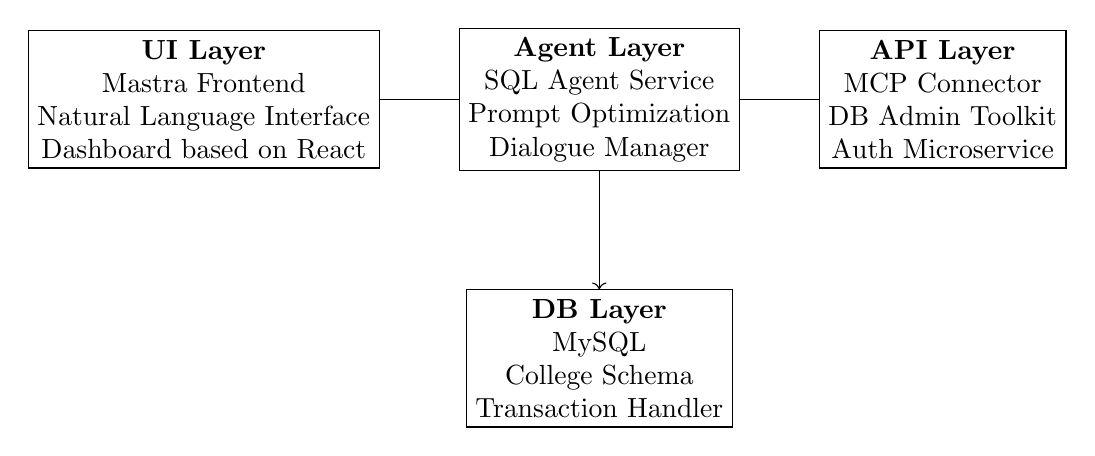
\begin{tikzpicture}[
			box/.style={
				draw, 
				rectangle,
				minimum width=2cm,
				minimum height=1cm,
				align=center
			}
			]
			
			% Left box
			\node[box] (left) {\textbf{UI Layer}\\Mastra Frontend\\Natural Language Interface\\Dashboard based on React};
			
			% Middle box
			\node[box, right=of left] (middle) {\textbf{Agent Layer}\\SQL Agent Service\\Prompt Optimization\\Dialogue Manager};
			
			% Right box
			\node[box, right=of middle] (right) {\textbf{API Layer}\\MCP Connector\\DB Admin Toolkit\\Auth Microservice};
			
			% Bottom box
			\node[box, below=1.5cm of middle] (bottom) {\textbf{DB Layer}\\MySQL\\College Schema\\Transaction Handler};
			
			% Optional: connect boxes with lines
			\draw[-] (left) -- (middle);
			\draw[-] (middle) -- (right);
			\draw[->] (middle) -- (bottom);
			
		\end{tikzpicture}
	\end{center}
	
	\section{项目代码结构解释}
	
	\subsection{UI layer - 前端界面}
	
	当前代码在apps/vite-react/src下,前端页面用react框架实现的GUI的形式呈现给用户,可以有更好的用户体验,快速上手本项目
	
	\begin{filetree}
        src/
        ├── App.tsx   # 项目页面呈现内容,包含背景、聊天框内容等
        ├── main.tsx  # 项目主入口
        ├── style.css # 前端css实现
	\end{filetree}
	
	\begin{tcolorbox}[
		title=关键能力,
		colback=white,
		colframe=blue!50,
		fonttitle=\bfseries,
		coltitle=black,
		breakable
		]Z
		\begin{itemize}
			\item[\textcolor{purple}{\textbullet}] \textbf{自然语言交互}:
			\begin{itemize}
				\item 智能输入建议与自动补全
				\item 多轮对话上下文保持
				\item 即时语法错误提示
			\end{itemize}
			
			\item[\textcolor{purple}{\textbullet}] \textbf{可视化展示}:
			\begin{itemize}
				\item SQL生成过程实时预览
				\item 查询结果智能渲染(表格/图表)
				\item 数据字段自动类型识别
			\end{itemize}
			
			\item[\textcolor{purple}{\textbullet}] \textbf{性能体验}:
			\begin{itemize}
				\item 本地缓存历史查询记录
				\item 大规模数据分页加载
				\item 异步非阻塞式交互
			\end{itemize}
			
			\item[\textcolor{purple}{\textbullet}] \textbf{安全控制}:
			\begin{itemize}
				\item 敏感操作二次确认
				\item 查询权限可视化提示
				\item 结果数据脱敏处理
			\end{itemize}
		\end{itemize}
	\end{tcolorbox}
	
	\subsection{API layer - MCP服务层}
	
	当前代码在package/mysql-mcp/src下,MCP服务层是数据库操作中间件,提供标准化访问接口与安全增强功能
	
	\begin{filetree}
        src/
        ├── index.js        # 服务启动入口
        ├── config/
        │   └── database.js # 连接配置中心
        └── tools/
        │   └── mysql-tools.js # 核心功能实现
        └── utils/
            ├── logger.js   # 日志
            ├── pagination.js  # 分页
            └── security.js # 安全
	\end{filetree}
	
	\begin{tcolorbox}[
		title=关键能力,
		colback=white,
		colframe=blue!50,
		fonttitle=\bfseries,
		coltitle=black,
		breakable
		]
		\begin{itemize}
			\item[\textcolor{filecolor}{\textbullet}] \textbf{安全增强}:所有查询自动进行参数化处理
			\item[\textcolor{filecolor}{\textbullet}] \textbf{元数据服务}:可视化获取数据库Schema
			\item[\textcolor{filecolor}{\textbullet}] \textbf{性能优化}:自动分页+查询缓存
			\item[\textcolor{filecolor}{\textbullet}] \textbf{审计追踪}:完整记录查询历史
			
			\medskip
			\textcolor{funccolor}{\texttt{核心工具函数}}:
			\begin{itemize}
				\item \texttt{mysqlQueryTool} - 带注入防护的查询执行
				\item \texttt{mysqlSchemaTool} - 表结构探查
				\item \texttt{paginationTool} - 智能结果分页
			\end{itemize}
		\end{itemize}
	\end{tcolorbox}
	
	\subsection{Agent Layer - AI代理层}
	
	当前代码在apps/express-server/src下,MCP服务层是数据库操作中间件,提供标准化访问接口与安全增强功能
	
	\begin{filetree}
        src/
        ├── agents/                  # AI代理实现
        │   └── mysql-agent.ts       # MySQL智能代理核心逻辑
        ├── mcp/                     # 模型控制协议
        │   └── index.ts             # MCP服务入口
        ├── model/                   # 大模型配置
        │   └── index.ts             # 模型参数管理
        └── prompts/                 # Prompt工程
        └── mysql-agent-prompt.ts # SQL生成专用Prompt模板
	\end{filetree}
	
	\begin{tcolorbox}[
		title=关键能力,
		colback=white,
		colframe=blue!50,
		fonttitle=\bfseries,
		coltitle=black,
		breakable
		]
		\begin{itemize}
			\item[\textcolor{filecolor}{\textbullet}] \textbf{NLP2SQL转换}:自然语言到SQL的智能转换
			\item[\textcolor{filecolor}{\textbullet}] \textbf{上下文感知}:多轮对话状态管理
			\item[\textcolor{filecolor}{\textbullet}] \textbf{模型集成}:通义千问大模型深度适配
			\item[\textcolor{filecolor}{\textbullet}] \textbf{Prompt工程}:动态提示优化技术
			
			\medskip
			\textcolor{funccolor}{\texttt{核心模块}}:
			\begin{itemize}
				\item \texttt{mysql-agent.ts} - SQL生成与验证
				\item \texttt{model/index.ts} - 大模型参数配置
				\item \texttt{mysql-agent-prompt.ts} - 动态提示模板引擎
			\end{itemize}
		\end{itemize}
	\end{tcolorbox}
	
	\subsection{运行流程}
	
	\begin{enumerate}[leftmargin=*,label=\textcolor{stepcolor}{\bfseries 步骤 \arabic*.}]
		\item \textbf{用户输入}:
		\textcolor{notecolor}{根据README配置并运行程序,进入Web界面接收自然语言查询请求}
		
		\item \textbf{语义解析}:
		\textcolor{notecolor}{MySQL Agent进行意图识别和实体提取}
		
		\item \textbf{元数据获取}:
		\textcolor{notecolor}{通过MCP SchemaTool查询数据库表结构}
		
		\item \textbf{SQL生成}:
		\textcolor{notecolor}{结合Prompt模板和对话上下文生成候选SQL}
		
		\item \textbf{安全审查}:
		\textcolor{notecolor}{MCP服务器执行语法检查和安全验证}
		
		\item \textbf{查询执行}:
		\textcolor{notecolor}{通过连接池执行SQL并记录审计日志}
		
		\item \textbf{结果交付}:
		\textcolor{notecolor}{将数据转换为可视化图表并提供查询优化建议}
	\end{enumerate}
	
	\section{MCP功能增强任务}
	
	\subsection{查询日志记录 /logs}
	
	\textbf{实现内容:}
	
	\begin{enumerate}[noitemsep, label={{\arabic*})}]
		\item 记录下用户查询的自然语言转化后的SQL语句
		\item 记录查询是否成功,成功则返回结果数量,失败则记录失败原因
	\end{enumerate}\textbf{}
	
	\textbf{代码实现逻辑}
	
	\begin{lstlisting}[language=Java, title=日志实现逻辑, tabsize=4]
    // 记录查询日志
    export function logQuery(sql, params = [], result = null, error = null) {
    	const timestamp = new Date().toISOString();
    	const logEntry = {
    		timestamp,
    		sql,
    		params,
    		success: !error,
    		resultCount: result ? (Array.isArray(result) ? result.length : 1) : 0,
    		error: error ? error.message : null
    	};
    	
    	const logLine = JSON.stringify(logEntry) + '\n';
    	
    	try {
    		fs.appendFileSync(logFile, logLine);
    	} catch (err) {
    		console.error('写入日志失败:', err);
    	}
    }
    
    // 获取查询日志
    export function getQueryLogs(limit = 100) {
    	try {
    		if (!fs.existsSync(logFile)) {
    			return [];
    		}
    		
    		const content = fs.readFileSync(logFile, 'utf8');
    		const lines = content.trim().split('\n').filter(line => line);
    		
    		return lines
    		.slice(-limit)
    		.map(line => {
    			try {
    				return JSON.parse(line);
    			} catch {
    				return null;
    			}
    		})
    		.filter(log => log !== null)
    		.reverse(); // 最新的在前
    	} catch (error) {
    		console.error('读取日志失败:', error);
    		return [];
    	}
    }
	\end{lstlisting}
	
	\begin{figure}[H]
		\centering
		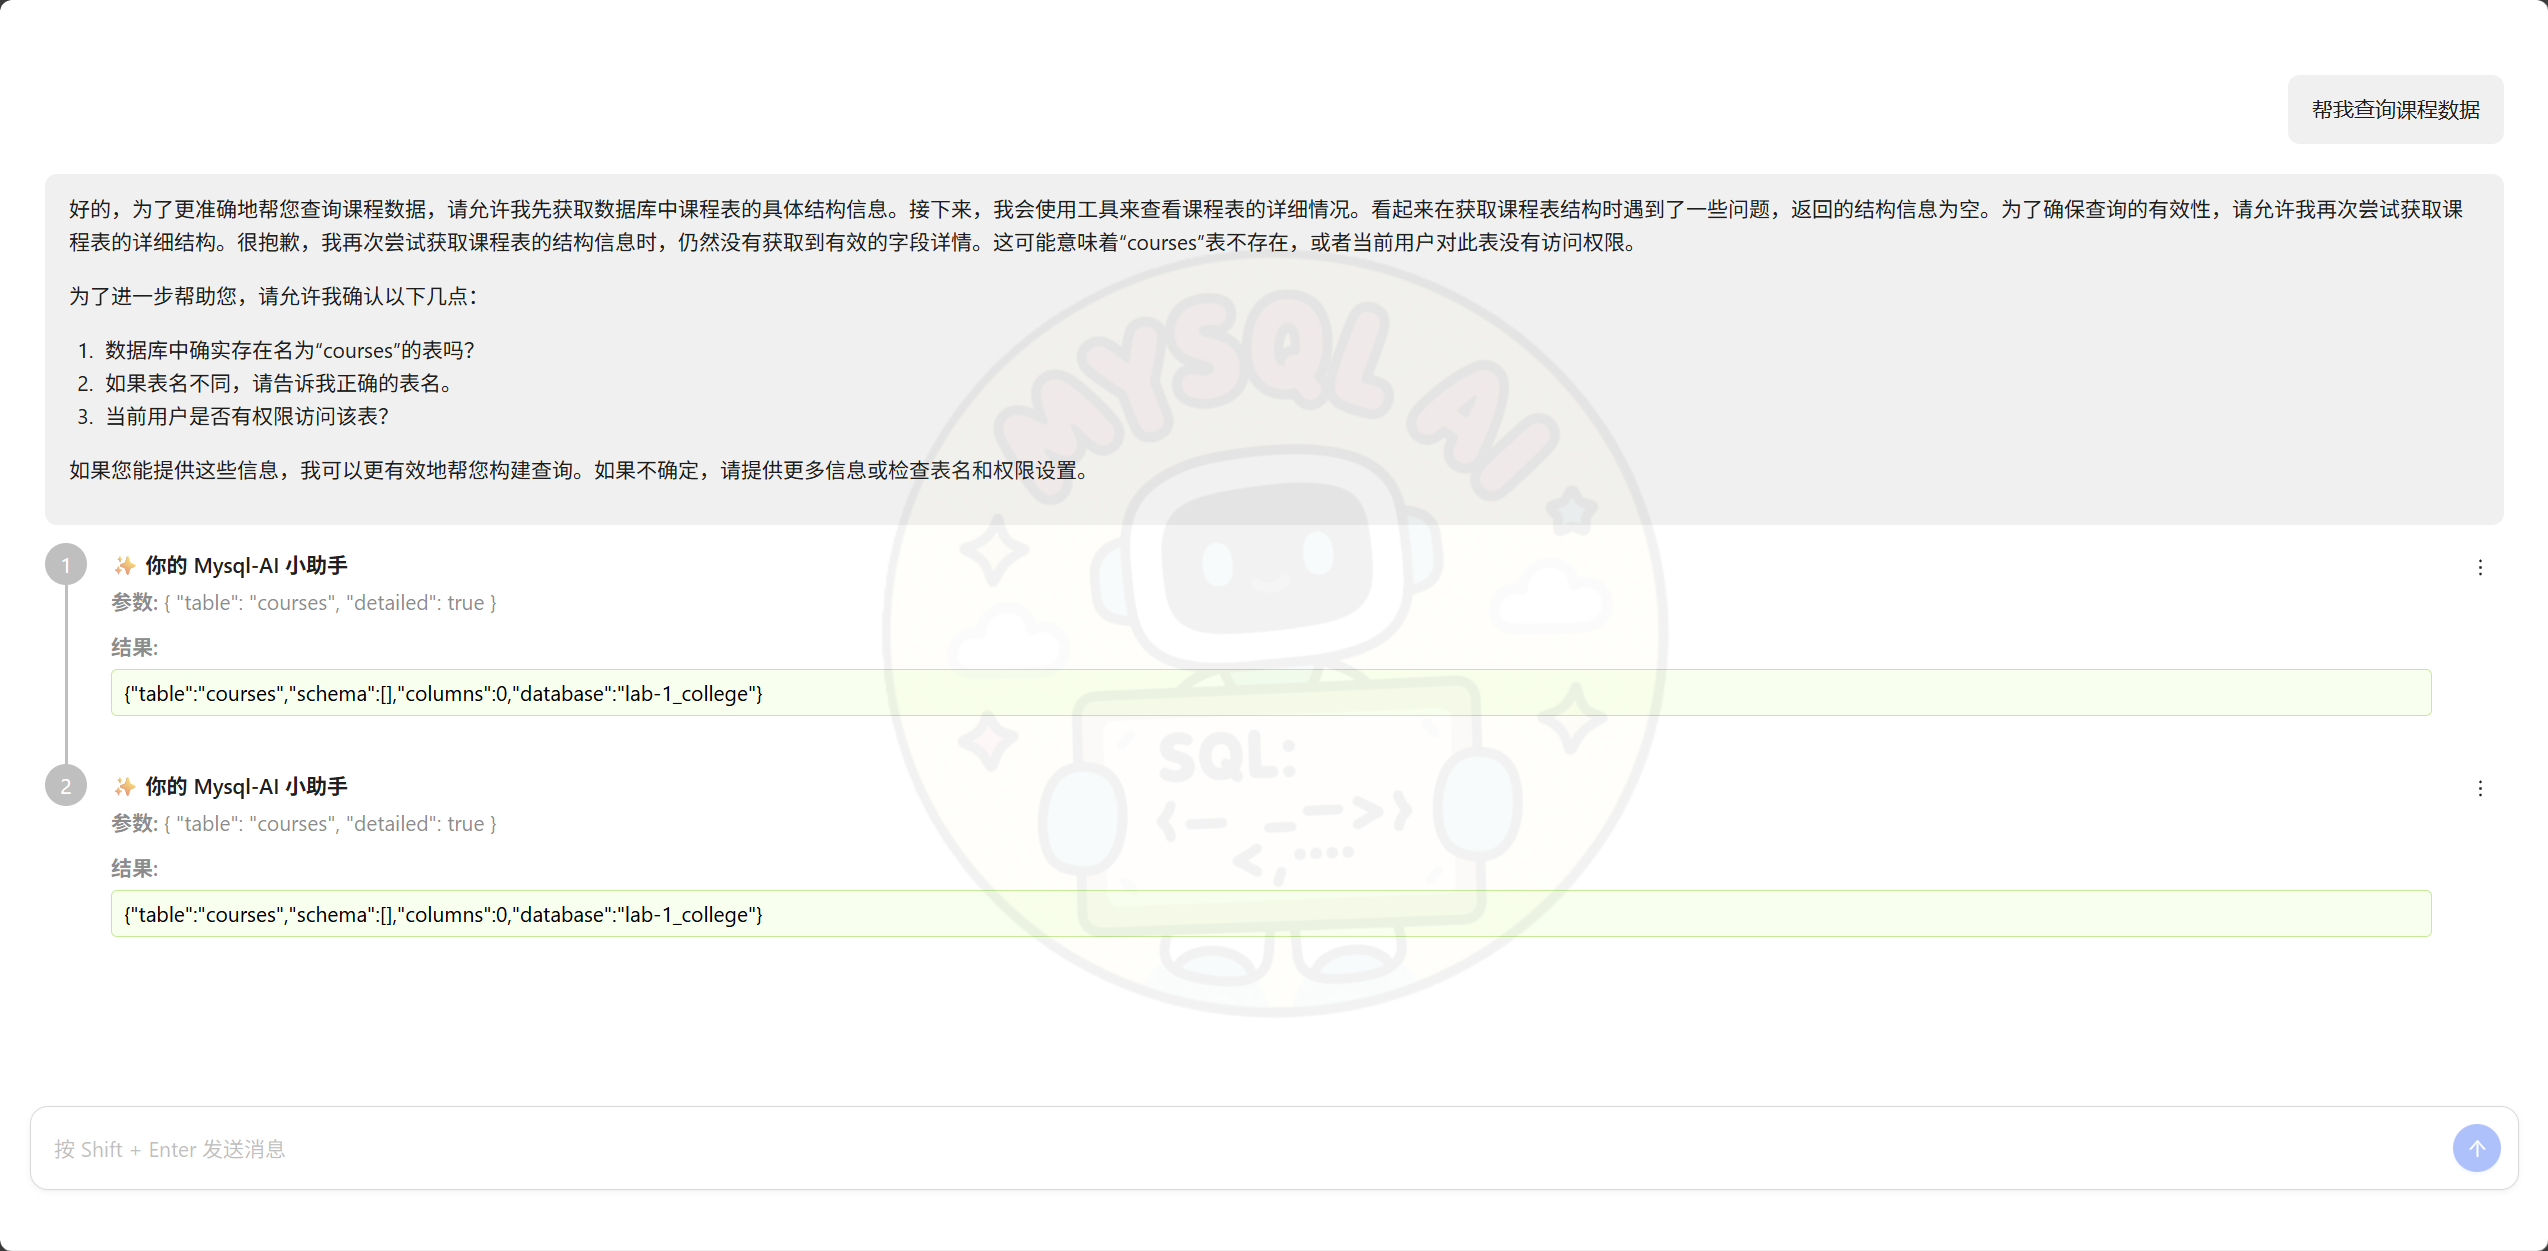
\includegraphics[width=17cm]{./images/1.日志.png}
		\caption{聊天日志截屏}
	\end{figure}
	
	\textbf{logs记录结构示例}
	
	\begin{lstlisting}[title=logs记录结构示例, tabsize=4]
    {
    	"timestamp":"2025-06-10T16:10:15.653Z",
    	"sql":"获取所有表信息",
    	"params":["lab-1_college"],
    	"success":true,
    	"resultCount":12,
    	"error":null
    },
    {
    	"timestamp":"2025-06-12T08:58:02.191Z",
    	"sql":"SELECT id, name, description, credits FROM courses LIMIT 100",
    	"params":[],
    	"success":false,
    	"resultCount":0,
    	"error":"SQL语句不是只读查询,仅允许SELECT和SHOW语句"
    },
	\end{lstlisting}
	
	\subsection{查询结果分页}
	
	\begin{enumerate}[noitemsep, label={{\arabic*})}]
		\item 页面上一次性显示更少的内容,优化用户体验
		\item 减少页面加载时间,减少内存占用
	\end{enumerate}\textbf{}
	
	\textbf{代码实现逻辑}
	
	\begin{lstlisting}[language=java, title=结果分页代码逻辑, tabsize=4]
    // 创建分页结果
    export function createPaginatedResult(results, pageSize = DEFAULT_PAGE_SIZE, sessionId = 'default') {
    	if (!Array.isArray(results)) {
    		return { data: results, pagination: null };
    	}
    	
    	pageSize = Math.min(pageSize, MAX_PAGE_SIZE);
    	
    	if (results.length <= pageSize) {
    		return { data: results, pagination: null };
    	}
    	
    	// 存储完整结果到分页状态
    	paginationStates.set(sessionId, {
    		results,
    		pageSize,
    		currentPage: 1,
    		totalPages: Math.ceil(results.length / pageSize),
    		totalItems: results.length
    	});
    	
    	const firstPageData = results.slice(0, pageSize);
    	return {
    		data: firstPageData,
    		pagination: {
    			currentPage: 1,
    			totalPages: Math.ceil(results.length / pageSize),
    			totalItems: results.length,
    			pageSize,
    			hasNext: results.length > pageSize,
    			hasPrevious: false
    		}
    	};
    }
    
    // 获取下一页
    export function getNextPage(sessionId = 'default') {
    	···
    }
    
    // 获取上一页
    export function getPreviousPage(sessionId = 'default') {
    	···
    }
    
    // 跳转到指定页
    export function goToPage(pageNumber, sessionId = 'default') {
    	const state = paginationStates.get(sessionId);
    	
    	if (!state) {
    		throw new Error('没有找到分页状态,请先执行查询');
    	}
    	
    	if (pageNumber < 1 || pageNumber > state.totalPages) {
    		throw new Error(`页码超出范围,有效范围: 1-${state.totalPages}`);
    	}
    	
    	state.currentPage = pageNumber;
    	const startIndex = (pageNumber - 1) * state.pageSize;
    	const endIndex = startIndex + state.pageSize;
    	const pageData = state.results.slice(startIndex, endIndex);
    	
    	return {
    		data: pageData,
    		pagination: {
    			currentPage: pageNumber,
    			totalPages: state.totalPages,
    			totalItems: state.totalItems,
    			pageSize: state.pageSize,
    			hasNext: pageNumber < state.totalPages,
    			hasPrevious: pageNumber > 1
    		}
    	};
    }
    
    // 清除分页状态
    export function clearPaginationState(sessionId = 'default') {
    	paginationStates.delete(sessionId);
    }
    
    // 获取分页状态信息
    export function getPaginationInfo(sessionId = 'default') {
    	const state = paginationStates.get(sessionId);
    	
    	if (!state) {
    		return null;
    	}
    	
    	return {
    		currentPage: state.currentPage,
    		totalPages: state.totalPages,
    		totalItems: state.totalItems,
    		pageSize: state.pageSize,
    		hasNext: state.currentPage < state.totalPages,
    		hasPrevious: state.currentPage > 1
    	};
    }
	\end{lstlisting}
	
	\begin{figure}[H]
		\centering
		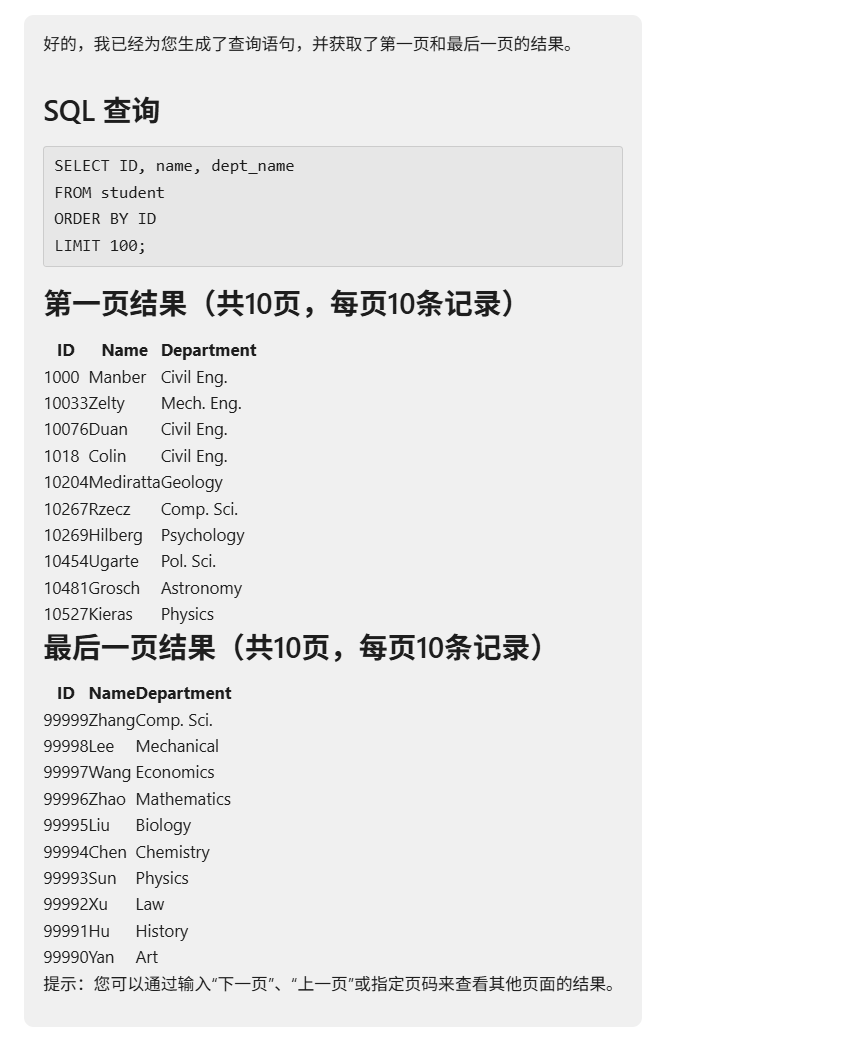
\includegraphics[width=11cm]{./images/2.分页.jpg}
		\caption{分页展示结果}
	\end{figure}
	
	\textbf{分页的数据结构:}
	
	\begin{lstlisting}[title=分页的数据结构, tabsize=4]
	{
		"data": [...],           // 当前页数据
		"pagination": {
			"currentPage": 1,
			"pageSize": 20,
			"totalRows": 150,
			"totalPages": 8,
			"hasNext": true,
			"hasPrev": false
		}
	}
	\end{lstlisting}
	
	\subsection{表结构简化输出}
	
	\textbf{实现内容:}
	
	\begin{enumerate}[noitemsep, label={{\arabic*})}]
		\item 用户可以按照需求获取自己需要的表的具体的、更精准的信息
		\item 减少了数据传输量,前端页面展示速率更快
	\end{enumerate}\textbf{}
	
	\textbf{代码实现逻辑:}
	
	\begin{lstlisting}[language=java, title=表结构简化代码, tabsize=4]
    // 创建获取表结构工具
    export const mysqlSchemaTool = createTool({
    	id: 'mysql_schema',
    	description: '获取数据库表结构信息,支持按表名过滤',
    	inputSchema: z.object({
    		table: z.string().optional().describe('表名,如果不提供则返回所有表'),
    		detailed: z.boolean().optional().describe('是否返回详细信息')
    	}),
    	execute: async ({ context }) => {
    		const { table, detailed = true } = context;
    		
    		try {
    			if (table) {
    				// 获取特定表结构
    				const result = await executeQuery(
    				SQL_TEMPLATES.TABLE_SCHEMA,
    				[config.database, table]
    				);
    				
    				logQuery(`获取表结构: ${table}`, [config.database, table], result);
    				
    				if (detailed) {
    					return { 
    						table: table,
    						schema: result,
    						columns: result.length,
    						database: config.database
    					};
    				} else {
    					// 简化输出
    					const simplified = result.map(col => ({
    						name: col.COLUMN_NAME,
    						type: col.COLUMN_TYPE,
    						nullable: col.IS_NULLABLE === 'YES',
    						key: col.COLUMN_KEY
    					}));
    					return { table: table, columns: simplified };
    				}
    			} else {
    				// 获取所有表信息
    				const result = await executeQuery(
    				SQL_TEMPLATES.ALL_TABLES,
    				[config.database]
    				);
    				
    				logQuery('获取所有表信息', [config.database], result);
    				
    				if (detailed) {
    					return { 
    						database: config.database,
    						tables: result,
    						tableCount: result.length
    					};
    				} else {
    					// 简化输出
    					const simplified = result.map(table => ({
    						name: table.TABLE_NAME,
    						type: table.TABLE_TYPE,
    						rows: table.TABLE_ROWS
    					}));
    					return { database: config.database, tables: simplified };
    				}
    			}
    		} catch (error) {
    			logQuery(`获取表结构失败: ${table || 'all'}`, [], null, error);
    			throw error;
    		}
    	}
    });
	\end{lstlisting}
	
	\begin{figure}[H]
		\centering
		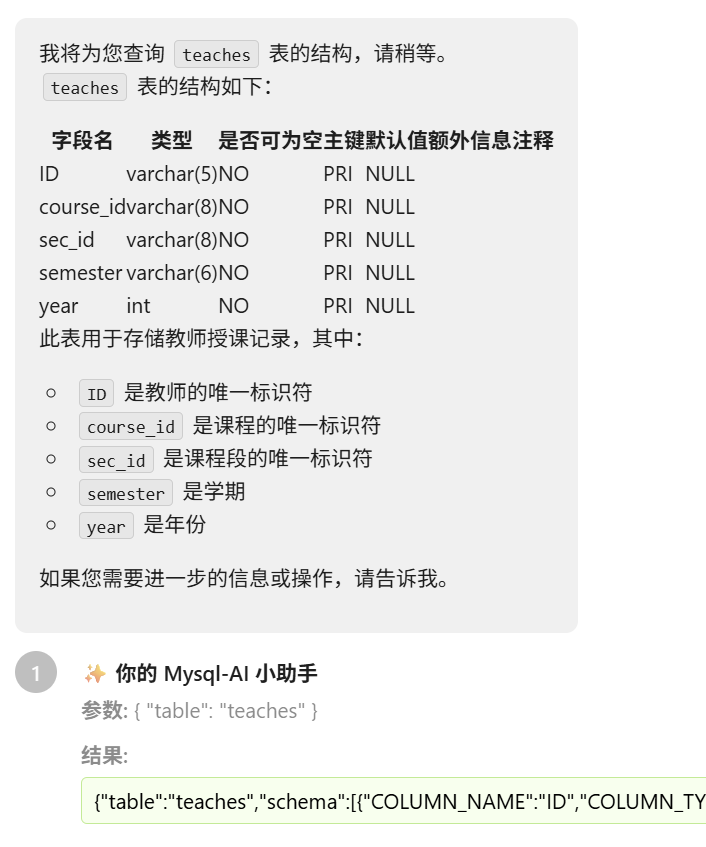
\includegraphics[width=11cm]{./images/3.简化表格.jpg}
		\caption{表结构简化输出}
	\end{figure}
	
	\section{MCP安全控制任务}
	
	\begin{lstlisting}[language=java, title=MCP安全检查, tabsize=4]
	// 综合安全检查
	export function validateSQL(sql) {
		// 检查是否为只读SQL
		if (!isReadOnlySQL(sql)) {
			return {
				valid: false,
				reason: 'SQL语句不是只读查询,仅允许SELECT和SHOW语句'
			};
		}
		
		// 检查敏感字段
		const sensitiveCheck = containsSensitiveFields(sql);
		if (sensitiveCheck.hasSensitiveField) {
			return {
				valid: false,
				reason: `禁止查询敏感字段: ${sensitiveCheck.field}`
			};
		}
		
		// 检查SQL注入
		const injectionCheck = detectSQLInjection(sql);
		if (injectionCheck.hasInjection) {
			return {
				valid: false,
				reason: `检测到潜在的SQL注入攻击: ${injectionCheck.type}`
			};
		}
		
		return { valid: true };
	}
	\end{lstlisting}
	
	\subsection{只读SQL白名单过滤}
	
	\textbf{实现代码示例:}
	
	\begin{lstlisting}[language=java, title=SQL白名单代码示例, tabsize=4]
	// 检查SQL是否为只读查询
	export function isReadOnlySQL(sql) {
		const cleanSQL = sql.trim().toUpperCase();
		
		// 只允许SELECT和SHOW语句
		if (!cleanSQL.startsWith('SELECT') && !cleanSQL.startsWith('SHOW')) {
			return false;
		}
		
		// 检查是否包含危险关键词
		for (const keyword of DANGEROUS_KEYWORDS) {
			if (cleanSQL.includes(keyword)) {
				return false;
			}
		}
		
		return true;
	}
	\end{lstlisting}
	
	\begin{figure}[H]
		\centering
		
\includegraphics[width=17cm]{./images/4.白名单.jpg}
		\caption{只读SQL白名单过滤}
	\end{figure}
	
	\subsection{关键字段访问控制}
	
	\begin{lstlisting}[language=java, title=关键字段查询控制, tabsize=4]
	// 敏感字段列表
	const SENSITIVE_FIELDS = [
		'password', 'passwd', 'pwd',
		'salary', 'income', 'wage',
		'ssn', 'social_security_number',
		'credit_card', 'card_number',
		'phone', 'email', 'address'
	];
	
	// 检查SQL中是否包含敏感字段
	export function containsSensitiveFields(sql) {
		const lowerSQL = sql.toLowerCase();
		
		for (const field of SENSITIVE_FIELDS) {
			if (lowerSQL.includes(field)) {
				return {
					hasSensitiveField: true,
					field: field
				};
			}
		}
		
		return { hasSensitiveField: false };
	}
	\end{lstlisting}
	
	\begin{figure}[H]
		\centering
		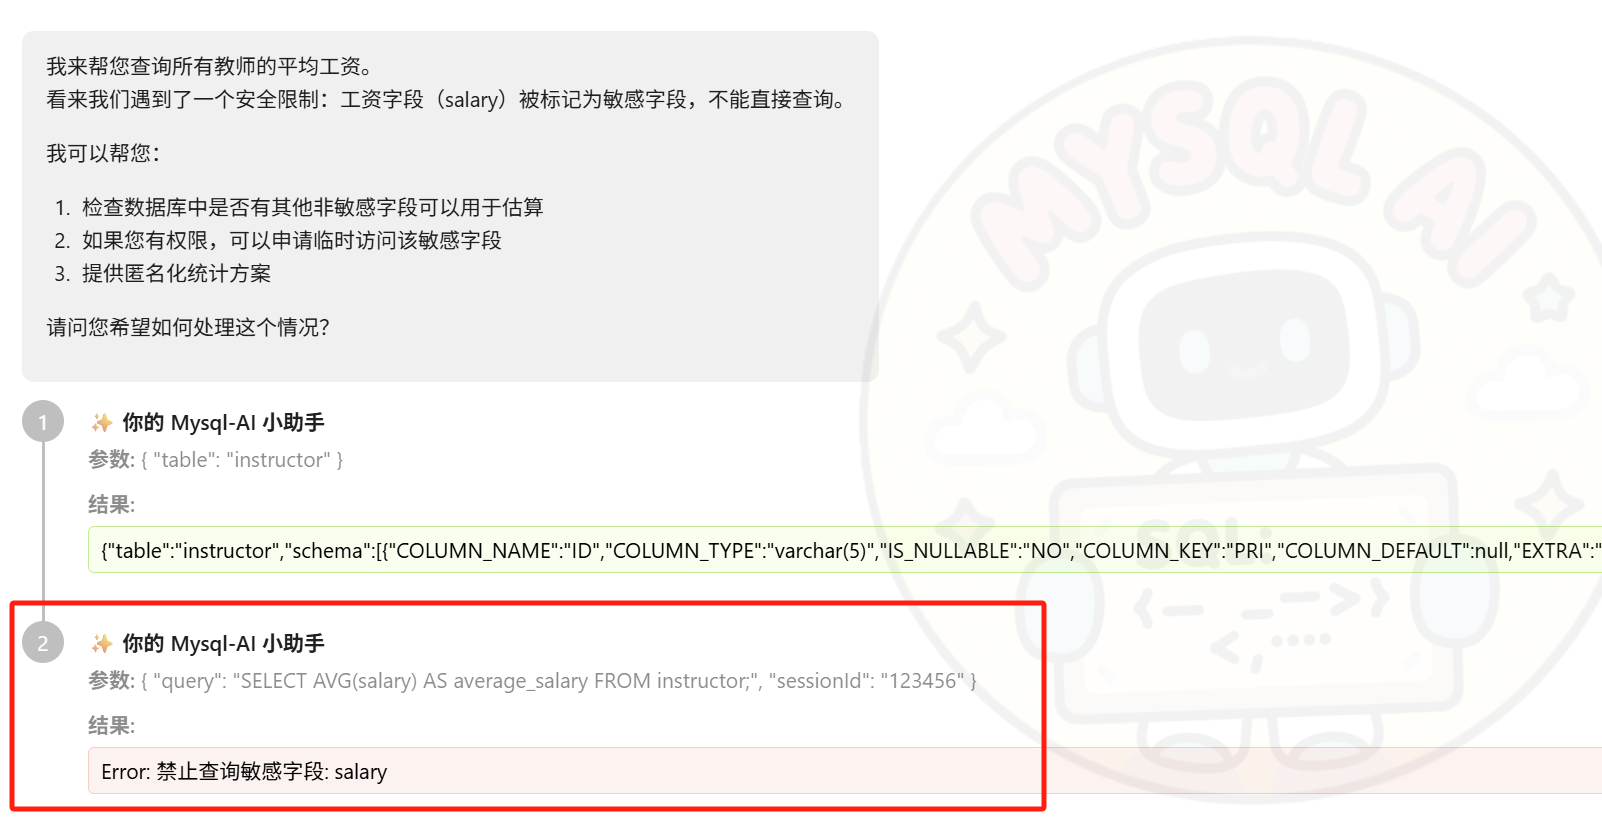
\includegraphics[width=15cm]{./images/5.敏感数据.jpg}
		\caption{关键字段访问控制}
	\end{figure}
	
	\subsection{简易SQL注入防御机制}
	
	\begin{lstlisting}[language=java, title=, tabsize=4]
	// SQL注入模式 - 移除SELECT检查,因为我们允许SELECT查询
	const INJECTION_PATTERNS = [
		/(''|\\|;|\/\*.*?\*\/|--.*$)/gim,
        /(exec(\s|\+)+(s|x)p\w+)/gi,
		/(\b(ALTER|CREATE|DELETE|DROP|EXEC|INSERT|MERGE|TRUNCATE)\b)/gi
	];
	
	// 检查SQL注入
	export function detectSQLInjection(sql) {
		// 检查明显的注入模式,但排除正常的SQL语法
		const suspiciousPatterns = [
		/(exec(\s|\+)+(s|x)p\w+)/gi,  // 存储过程执行
		/(\bunion\s+select)/gi,        // UNION SELECT攻击
		/(;\s*(drop|delete|insert|update))/gi  // 多语句攻击
		];
		
		for (const pattern of suspiciousPatterns) {
			if (pattern.test(sql)) {
				return {
					hasInjection: true,
					type: 'pattern_match',
					pattern: pattern.toString()
				};
			}
		}
		
		// 检查单引号不匹配(但允许正常的字符串)
		const singleQuotes = (sql.match(/''/g) || []).length;
		if (singleQuotes % 2 !== 0) {
			return {
				hasInjection: true,
				type: 'unmatched_quotes'
			};
		}
		
		// 检查多个分号(但允许单个分号结尾)
		const semicolons = (sql.match(/;/g) || []).length;
		const endsWithSemicolon = sql.trim().endsWith(';');
		if (semicolons > 1 || (semicolons === 1 && !endsWithSemicolon)) {
			return {
				hasInjection: true,
				type: 'multiple_statements'
			};
		}
		
		return { hasInjection: false };
	}
	\end{lstlisting}
	
	\begin{figure}[H]
		\centering
		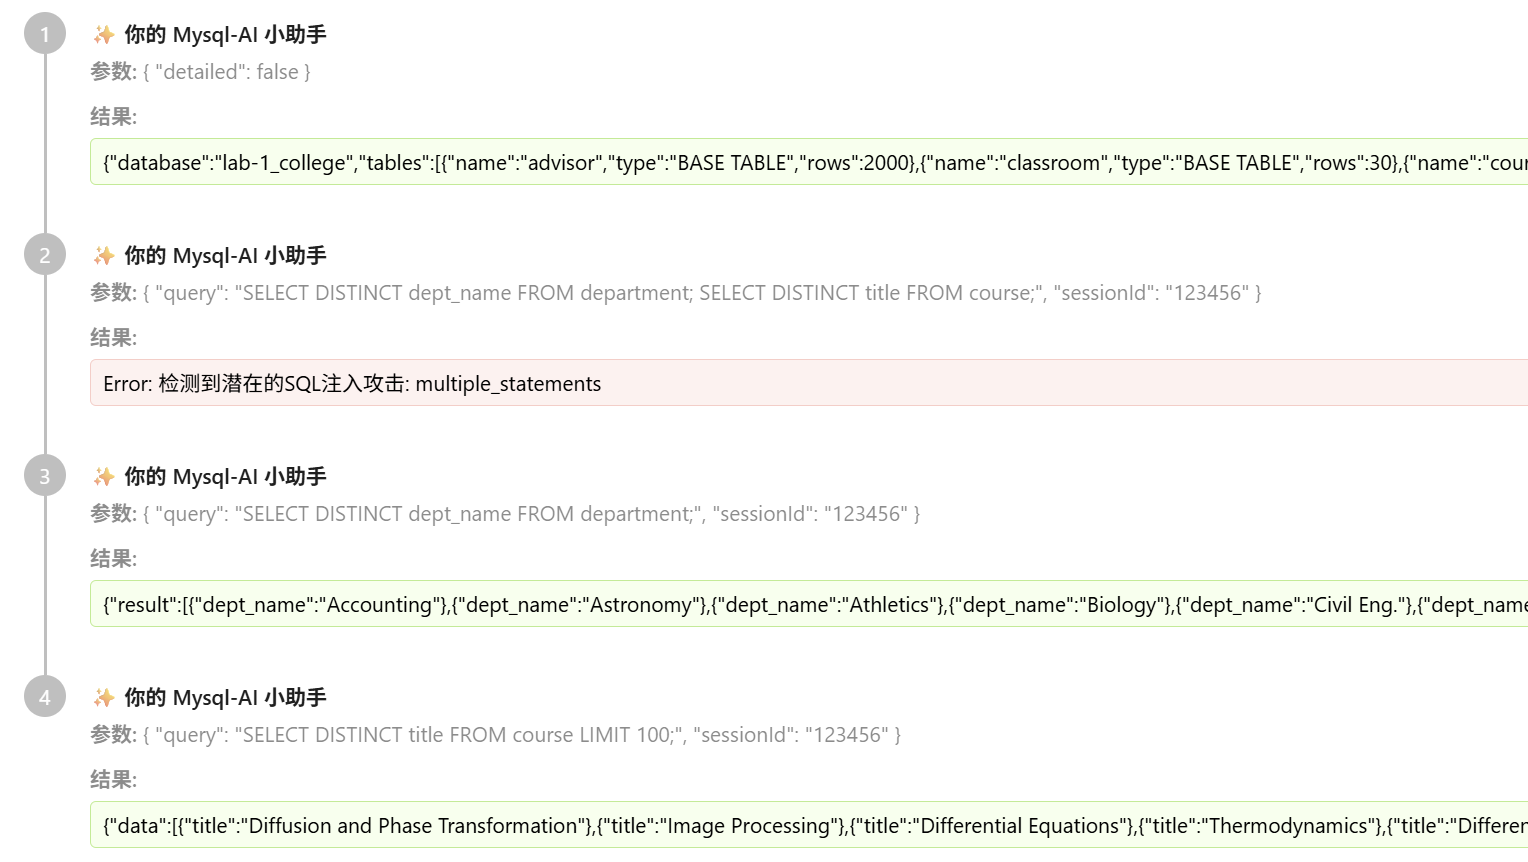
\includegraphics[width=13cm]{./images/6.SQL注入.png}
		\caption{简易SQL注入防御机制}
	\end{figure}
	
	\section{大模型优化任务/UI扩展任务}
	
	\subsection{Prompt模块优化}
	
	此处主要是利用提示词来告诉大模型需要如何操作我的指令
	
	当前文件的位置在apps/express-server/src/prompts/mysql-agent-prompts.ts
	
	\subsubsection{角色设定}
	
	\begin{lstlisting}[title=角色设定, tabsize=4]
	你是一个智能MySQL查询转换器,专门将用户的问题变成安全、高效的SQL查询。
	\end{lstlisting}
	
	\subsubsection{任务指令}
	
	\begin{lstlisting}[title=任务指令, tabsize=4]
	## 你的主要职责:
	1. **精准需求分析**
		- 自动识别用户查询中的关键要素(表名、字段、条件)
		- 对模糊表述要求用户确认(如"销量高的产品"需明确具体阈值)
		- 支持多轮对话中的指代消解(如"它们"指向前文提到的表)
	2. **安全SQL生成**
		- 严格基于数据库实时Schema生成查询
		- 所有查询必须包含显式字段列表(禁止SELECT *)
		- 自动添加LIMIT子句(默认100行,可调整)
		- 对潜在危险操作强制二次确认
	3. **智能结果处理**
		- 自动检测数据异常(空值、异常值、逻辑冲突)
		- 根据数据特征选择展示格式(表格/图表/统计摘要)
		- 对大数据集提供智能分页(保留上下文的分页查询)
	4. **持续性能优化**
		- 为每个查询提供索引建议
		- 标记潜在性能瓶颈(如全表扫描)
		- 建议查询改写方案(如用JOIN代替子查询)
		- 记录历史查询性能指标供对比参考
	\end{lstlisting}
	
	\subsubsection{规则约束}
	
	\begin{lstlisting}[title=规则约束, tabsize=4]
	## SQL生成规则:
	1. **查询安全控制**
		- 仅允许生成SELECT查询语句
		- 禁止包含数据修改操作(INSERT/UPDATE/DELETE/TRUNCATE)
		- 自动屏蔽敏感字段(密码、密钥等)
	2. **表连接规范**
		- 优先使用INNER JOIN明确关联关系
		- 必须指定连接条件(禁止笛卡尔积)
		- 多表连接时使用表别名提高可读性
		- 超过3个表连接时自动检查执行计划
	3. **数据过滤要求**
		- WHERE子句必须包含至少1个有效条件
		- 对字符串条件自动添加防注入处理
		- 日期范围查询必须明确上下界
	4. **结果集控制**
		- 默认添加LIMIT 100(可调整)
		- 超过10万行结果必须强制分页
		- 排序字段超过3列时提示性能风险
	5. **性能优化建议**
		- 为每个查询提供至少2条优化建议
		- 包含索引建议(基于WHERE/JOIN/ORDER BY字段)
		- 标记潜在的全表扫描风险
		- 建议查询重写方案(如可用CTE替代子查询)
	6. **代码风格要求**
		- 关键字全大写(SELECT/WHERE等)
		- 使用4空格缩进
		- 每个字段单独一行
		- 复杂查询必须包含注释说明
	\end{lstlisting}
	
	\subsection{多轮提示结构/示例增强Few-shot}
	
	\subsubsection{多轮提示结构}
	
	多轮提示结构的设计如下所示:
	
	\begin{lstlisting}[title=多轮提示结构, tabsize=4]
	用户: "查找所有名为 “李华” 的学生的课程名称和成绩。"
	助手: 正在为您查询李华同学的课程信息和成绩。
	SQL: SELECT c.name, e.grade FROM students s JOIN enrollments e ON s.id = e.student_id JOIN courses c ON e.course_id = c.id WHERE s.name = '李华';
	优化建议: 确保 student_id 和 course_id 字段有索引,以提高查询性能。
	
	用户: "再帮我查下教师的平均课程评分。"
	助手: 根据您的上文需求,补充查询教师的平均课程评分。
	SQL: SELECT t.name, AVG(e.grade) AS avg_score FROM teachers t JOIN courses c ON t.id = c.teacher_id JOIN enrollments e ON c.id = e.course_id GROUP BY t.name;
	优化建议: 可为 teacher_id 和 grade 字段建立索引,以提升查询效率。
	\end{lstlisting}
	
	\subsubsection{示例增强Few-shot}
	
	few-shot结构设计如下所示:
	
	\begin{lstlisting}[title=示例增强Few-shot, tabsize=4]
	## Few-shot 示例对话:
	用户: "列出所有教师的姓名和所在的系别,按系别和教师姓名排序。"
	助手: 我来帮您查询教师信息。首先,我需要获取数据库的结构,然后生成相应的 SQL 查询。
	SQL: SELECT name, department FROM teachers ORDER BY department, name;
	优化建议: 可为 department 和 name 字段建立索引,以提升排序效率。
	
	请始终使用可用的MCP工具来获取schema信息和执行查询。
	\end{lstlisting}
	
	\subsubsection{记忆功能}
	
	大模型可以根据用户最近提问的几条指令来做出相关的回答,可以让用户有更好的用户体验
	
	\begin{figure}[H]
		\centering
		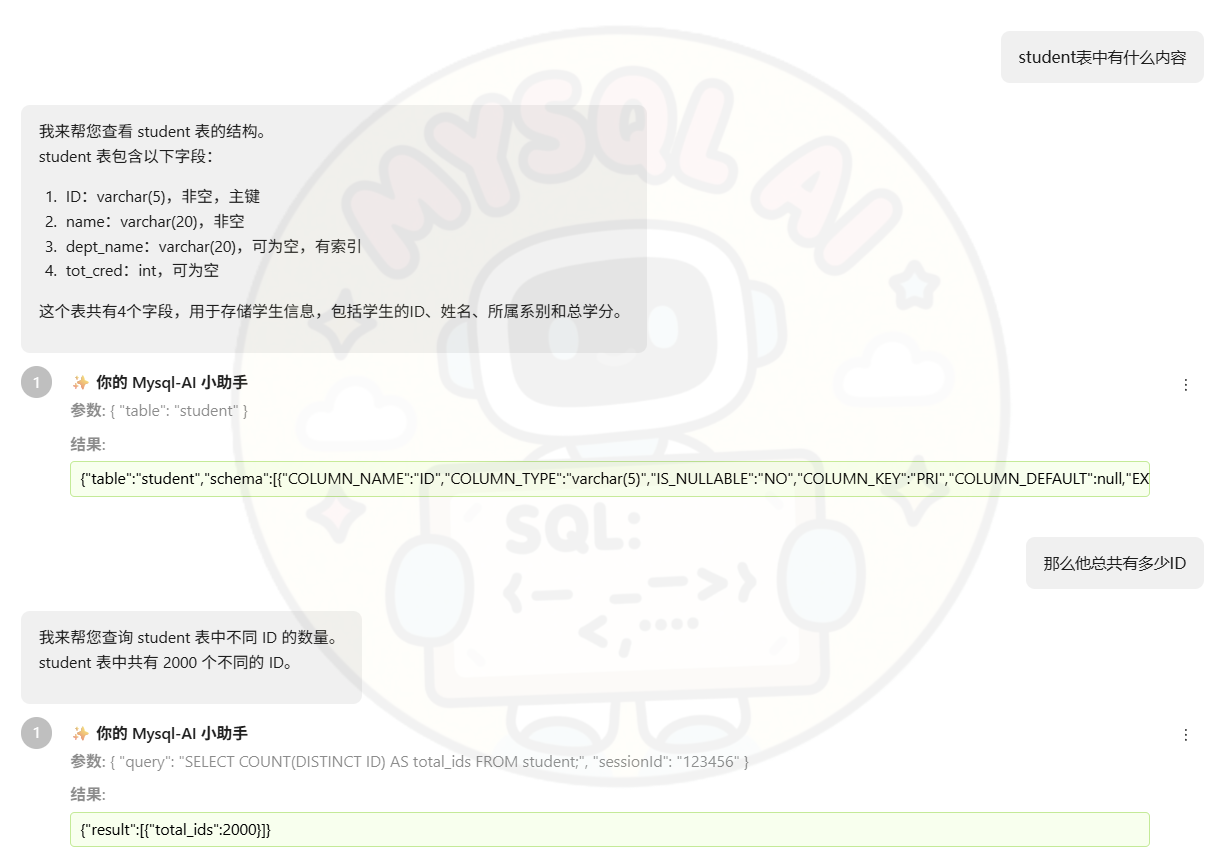
\includegraphics[width=13cm]{./images/7.记忆.jpg}
		\caption{记忆功能}
	\end{figure}
	
	\subsection{SQL执行计划简化建议}
	
	SQL执行语句与简化,以及其他约束条件如下所示:
	
	\begin{lstlisting}[title=SQL执行计划简化建议, tabsize=4]
	## 查询步骤:
	1. **获取数据库结构**
		- 强制使用工具获取最新表结构
		- 禁止任何自主猜测行为
	2. **分析查询需求**
		- 明确用户需要的字段和条件
		- 对模糊表述进行确认
	3. **生成执行SQL**
		- 包含6位会话ID标记
		- 使用标准Markdown代码块格式
		- 自动添加分页限制
	4. **解释与优化**
		- 用通俗语言说明查询结果
		- 提供至少1条可落地的优化建议
	
	## 语言
	如果用户没有明确使用哪种语言,你必须默认使用简体中文回答,即便用户使用英文和你对话,你也要用中文回答。
	例如:
	
	用户:"How many active users do we have?"
	助手:"好的,我将为您查询活跃用户数量。需要确认:
	- 您定义的'active user'是指最近30天有登录(login)的用户吗?
	- 需要区分用户类型(user type)吗?"
	
	
	## 输出限制
	1. **结果数量较多时(超过 30 条)**  
	- 返回前 10 条和后 10 条结果  
	- 提示用户总结果条数  
	2. **结果字段较多且结果集较小时**  
	- 以表格形式美观输出  
	3. **分页查询支持**  
	- 当上一轮输出结果较多时,如果用户继续查询(如:"下一页"、"next"、"翻页"、"第x页"等),使用 MCP 分页工具分页展示结果  
	\end{lstlisting}
	
	效果如下:
	
	\begin{figure}[H]
		\centering
		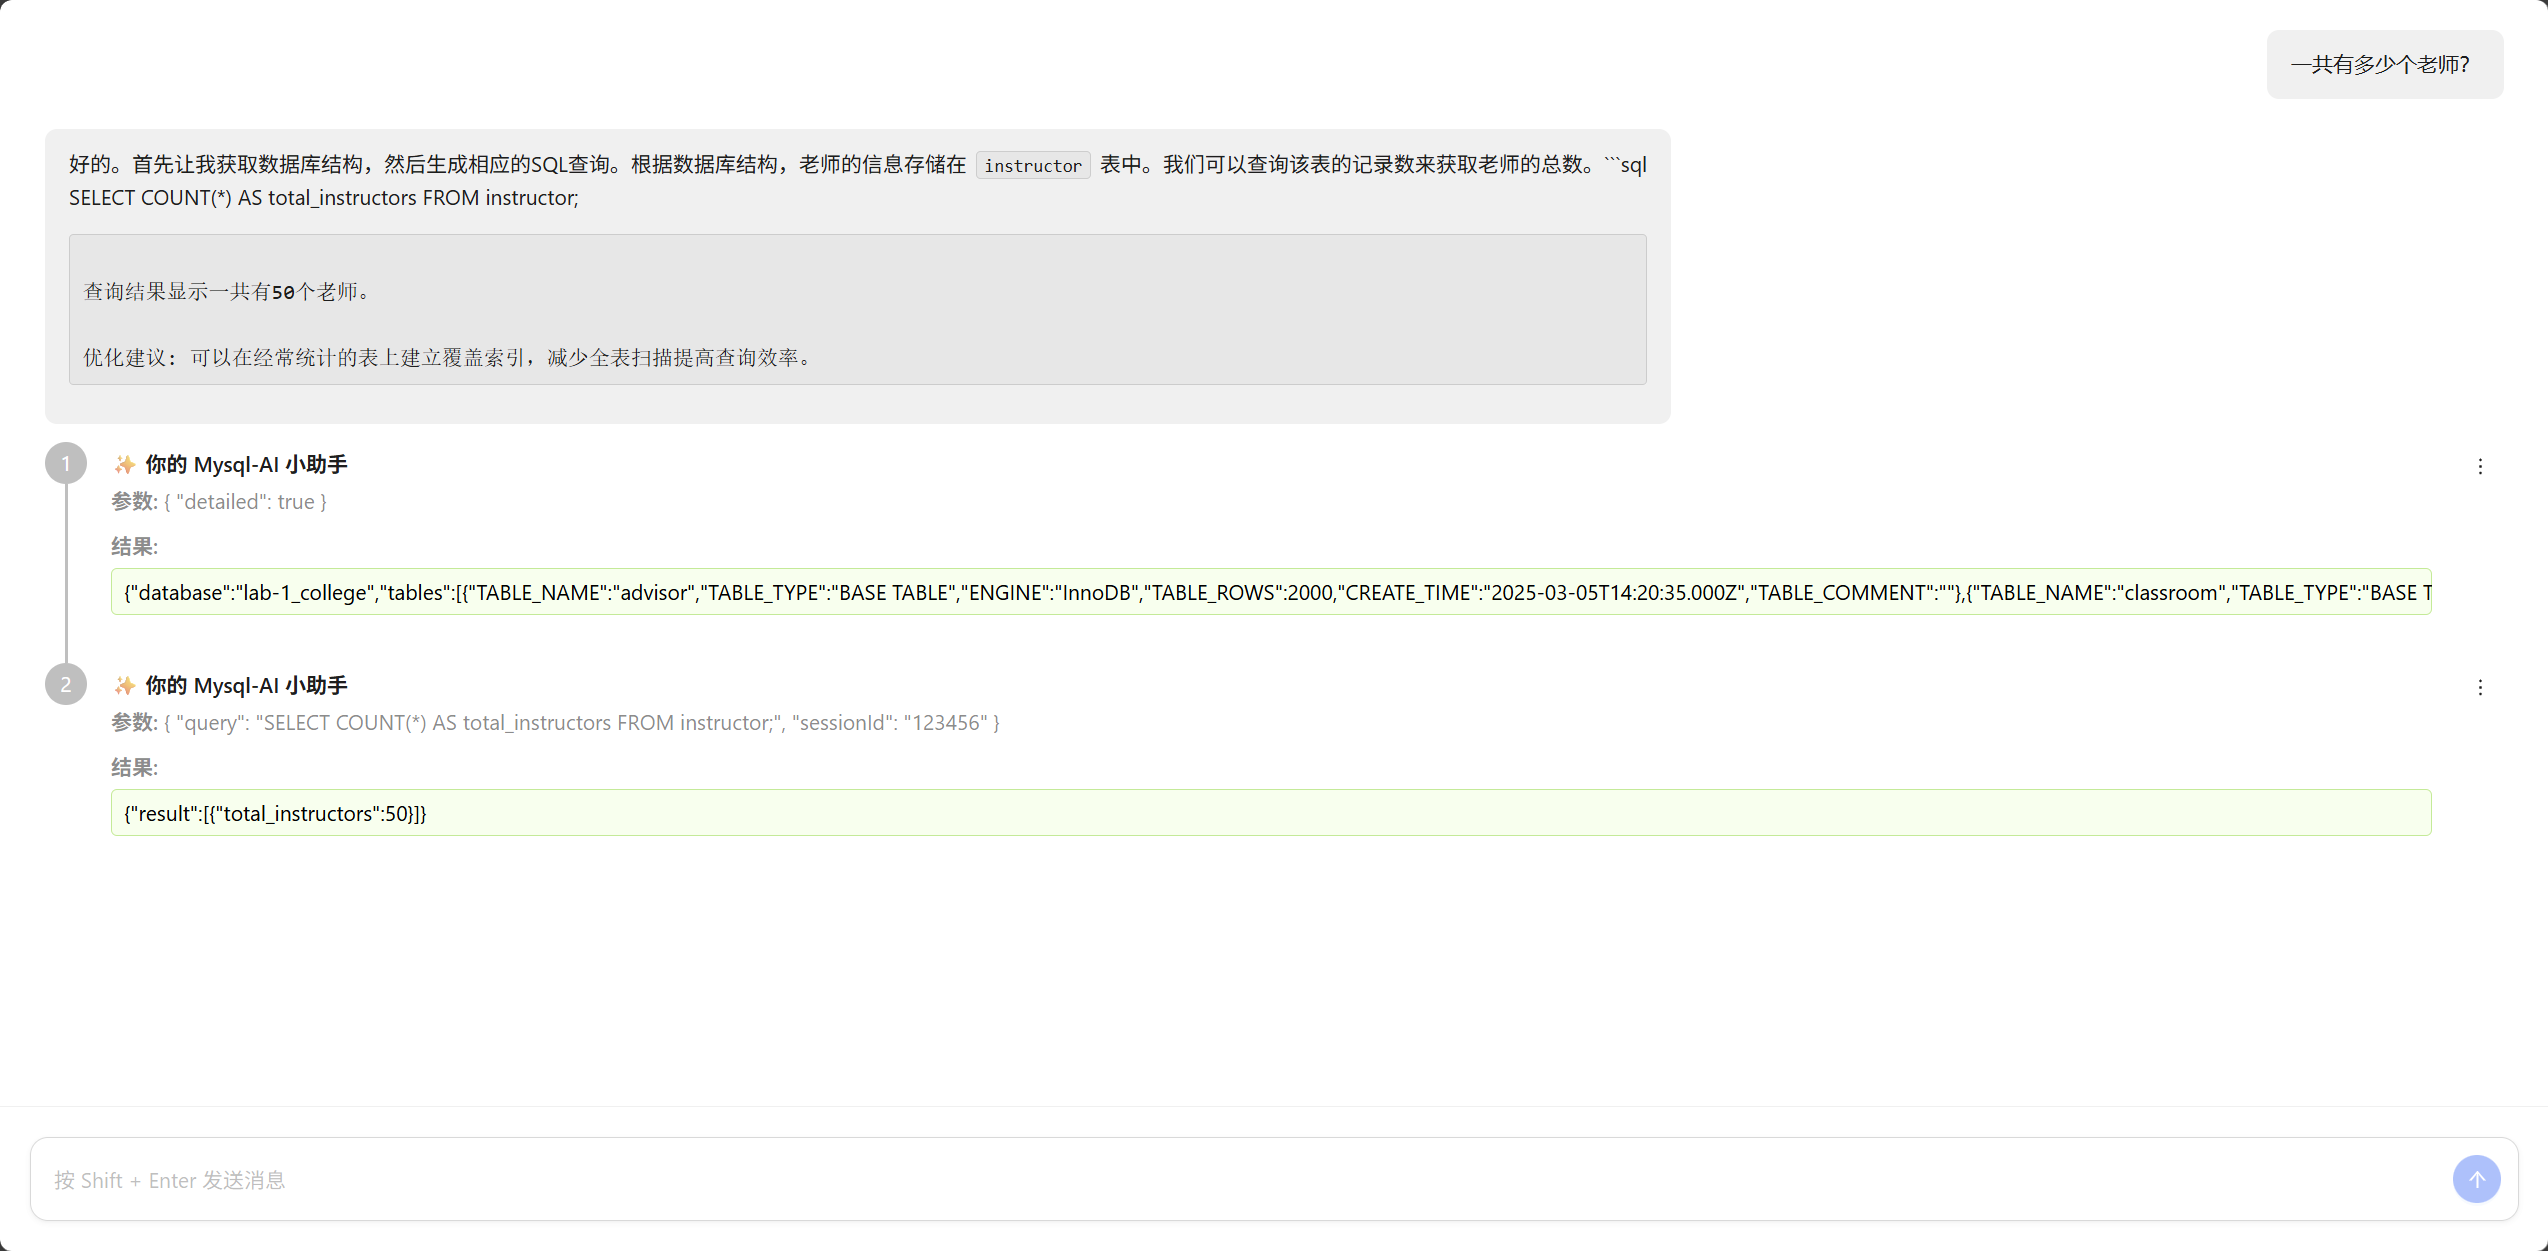
\includegraphics[width=15cm]{./images/8.优化建议.png}
		\caption{SQL执行语句与简化}
	\end{figure}
	
	\subsection{GUI界面}
	
	大部分GUI界面在前面已经显示,此处添加一张首页照片
	
	\begin{figure}[H]
		\centering
		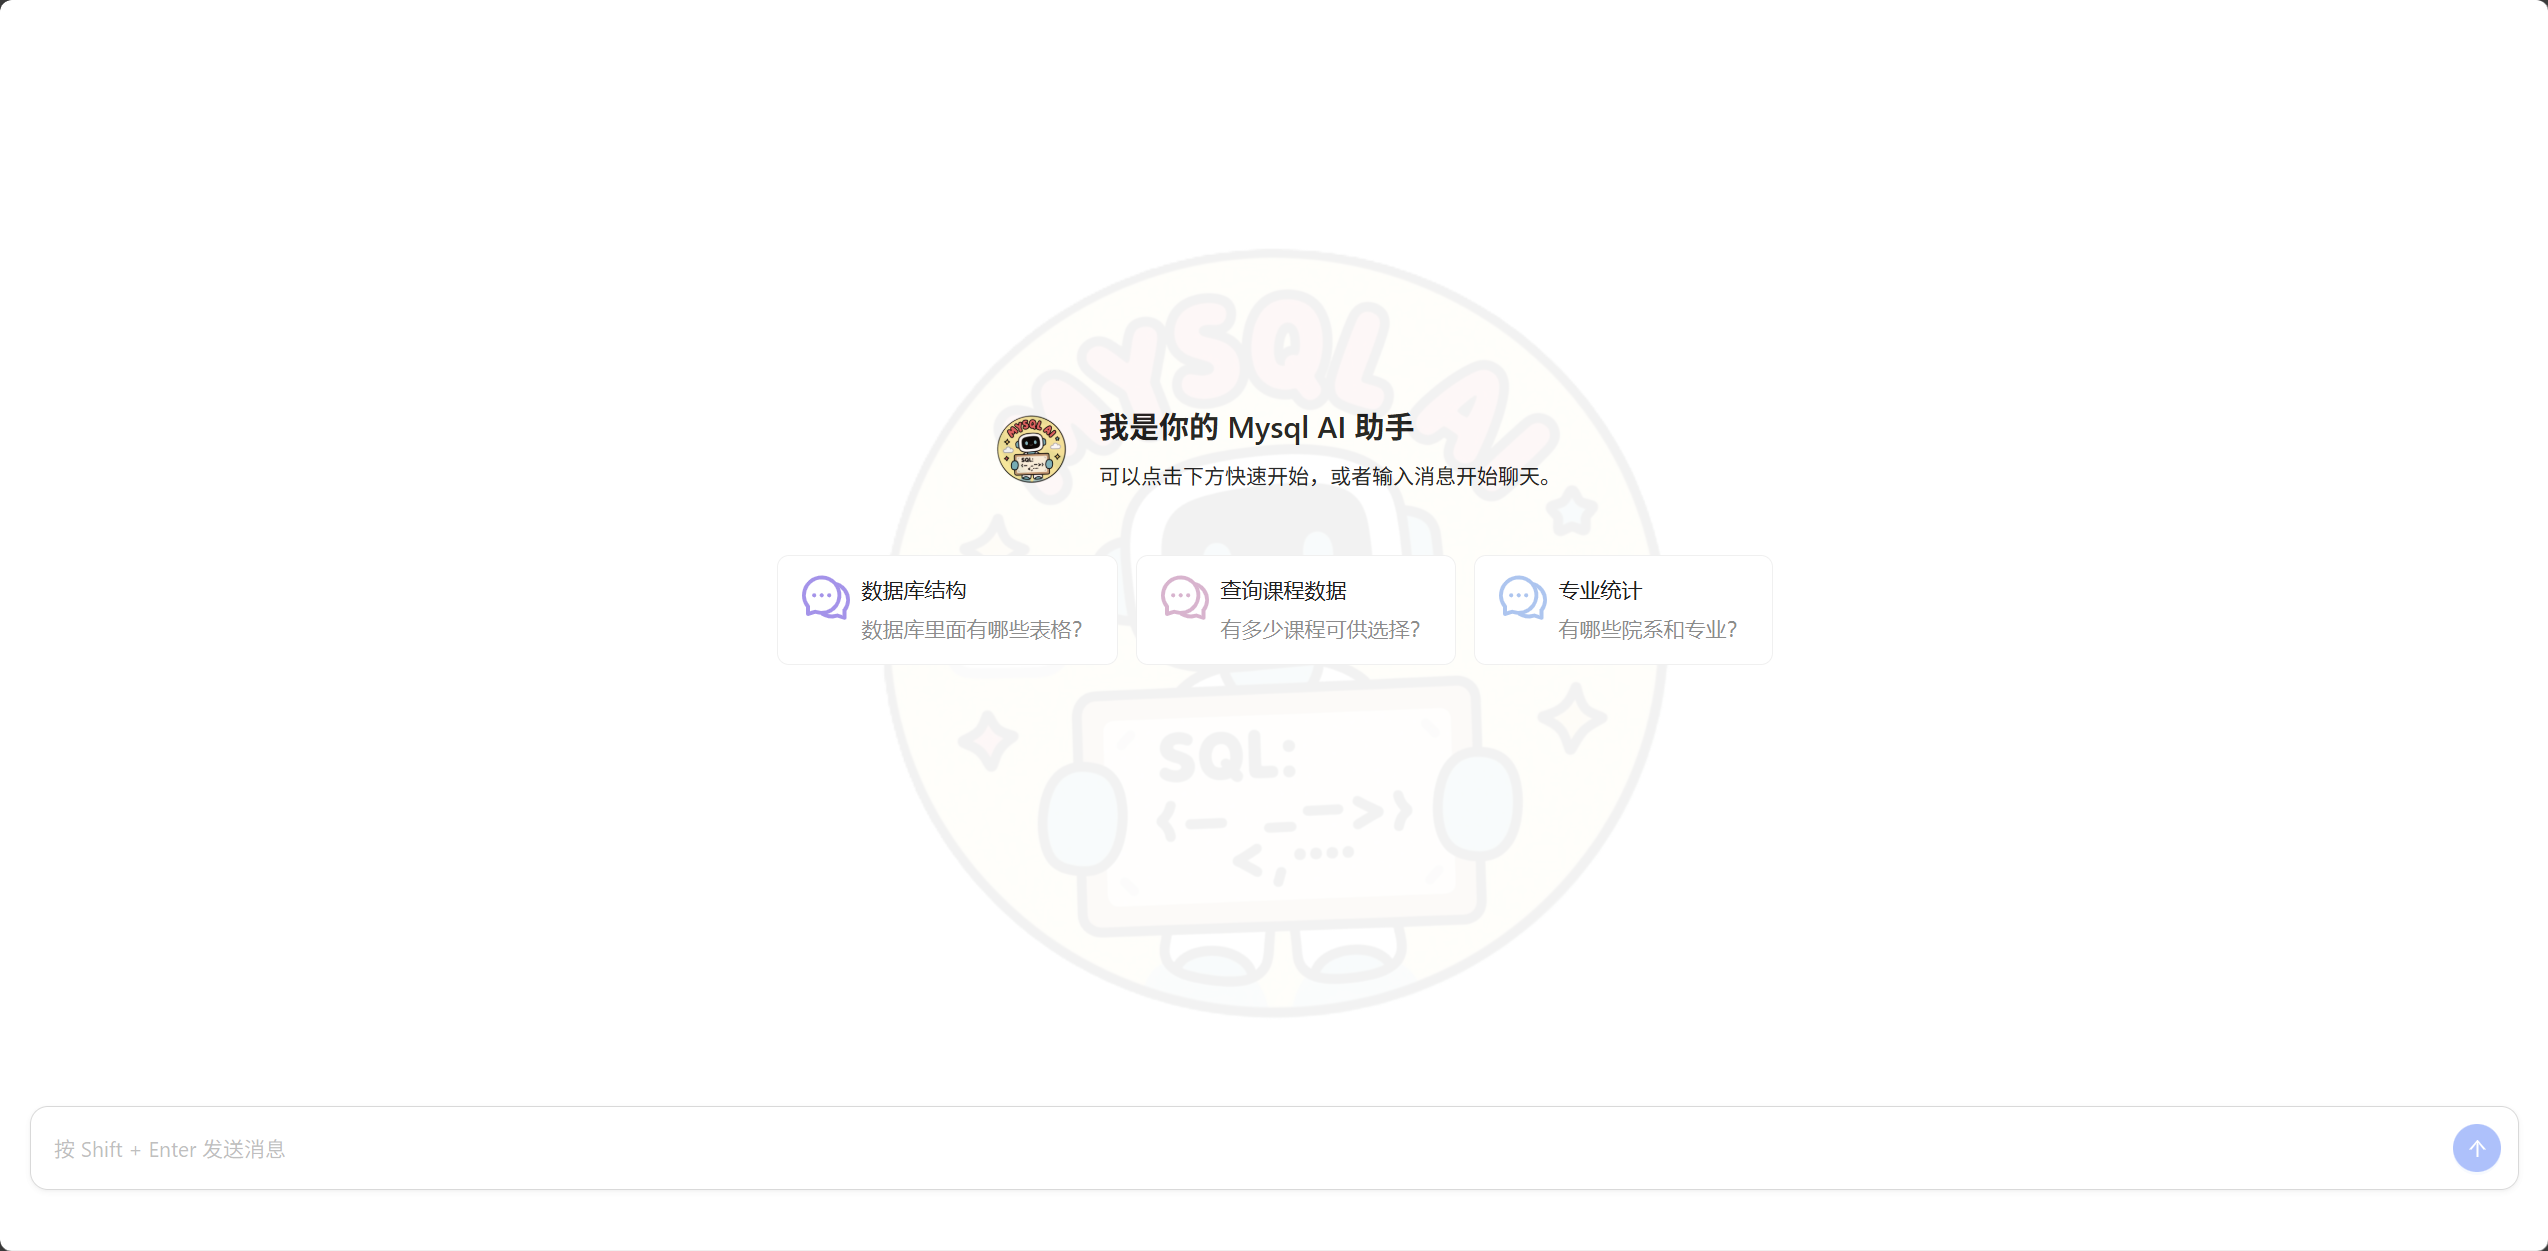
\includegraphics[width=15cm]{./images/9.GUI.png}
		\caption{GUI界面 - 首页}
	\end{figure}
	
	\section{测试用例}
	
	至此,所有的实验已经基本完成,现在来用第一次实验的题目来做一下测试,以验证准确性
	
	\begin{enumerate}[noitemsep, label={{\arabic*})}]
		\item List the names of all courses ordered by their titles and credits. 
		
		\begin{figure}[H]
			\centering
			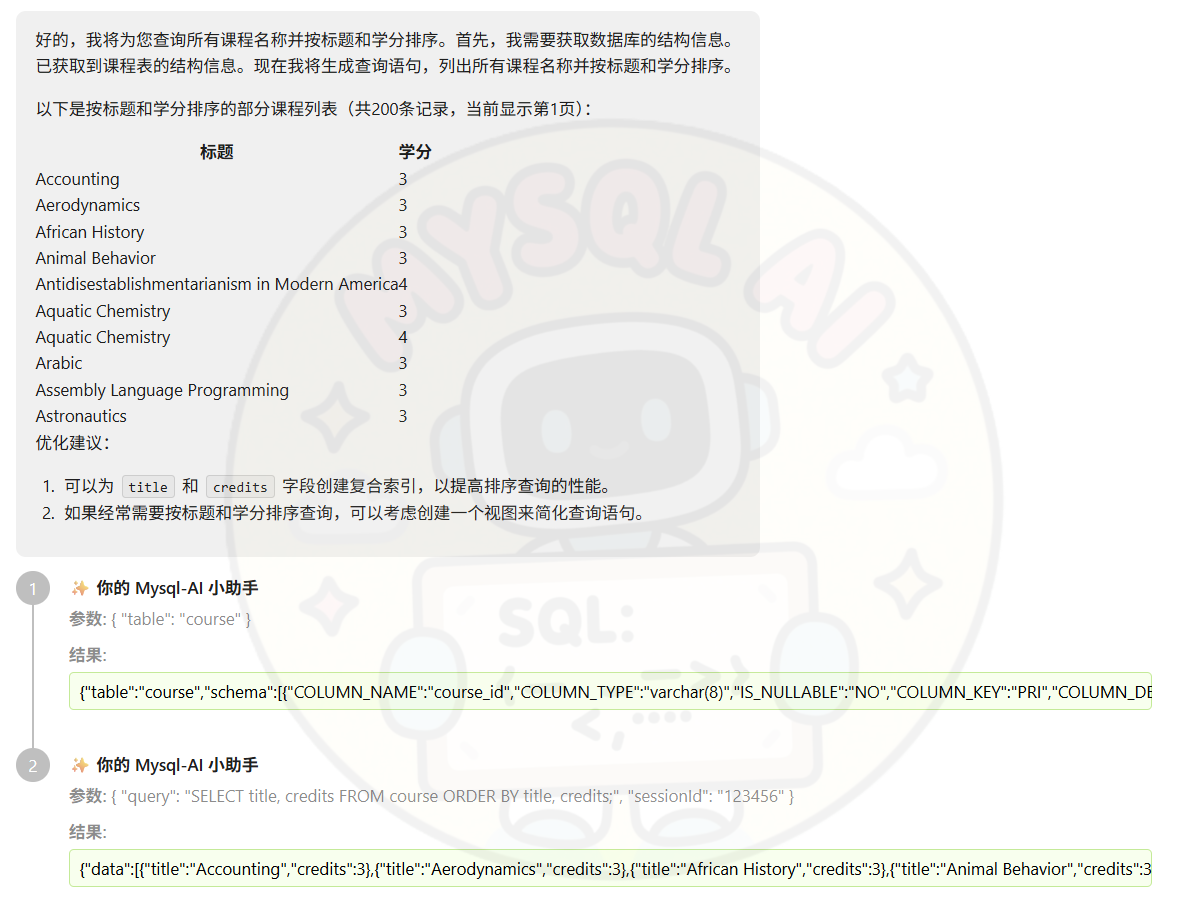
\includegraphics[width=10cm]{./images/10.测试1.jpg}
			\caption{测试1}
		\end{figure}
		
		\item What is the title, credit value, and department name for courses with more than one prerequisite?
		
		\begin{figure}[H]
			\centering
			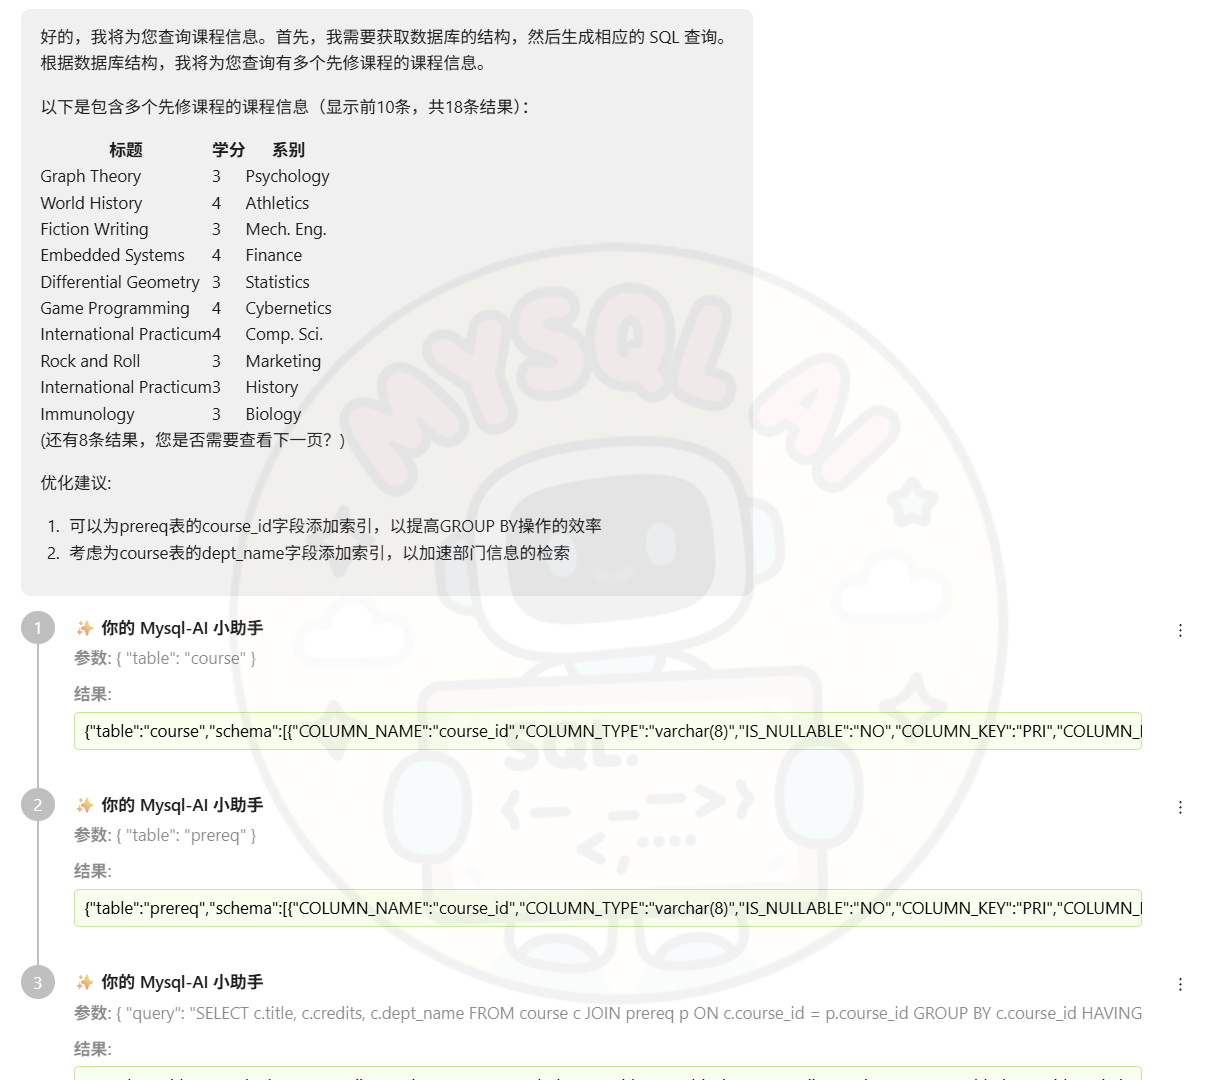
\includegraphics[width=10cm]{./images/11.测试2.jpg}
			\caption{测试2}
		\end{figure}
		
		\item What are the names of students who have more than one advisor?
		
		\begin{figure}[H]
			\centering
			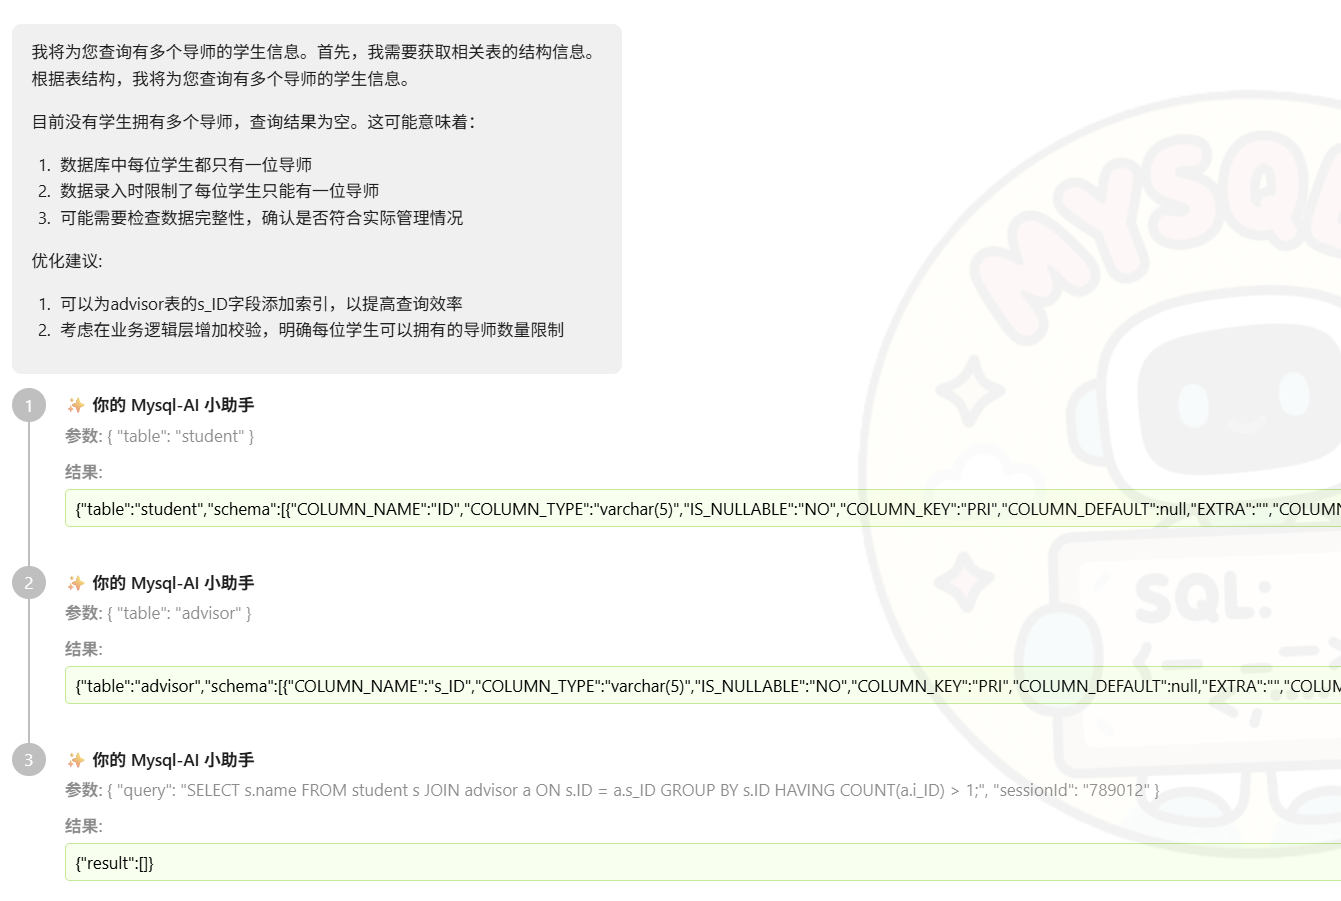
\includegraphics[width=10cm]{./images/12.测试3.jpg}
			\caption{测试3}
		\end{figure}
		
		\item What are the titles of courses without prerequisites? 
		
		\begin{figure}[H]
			\centering
			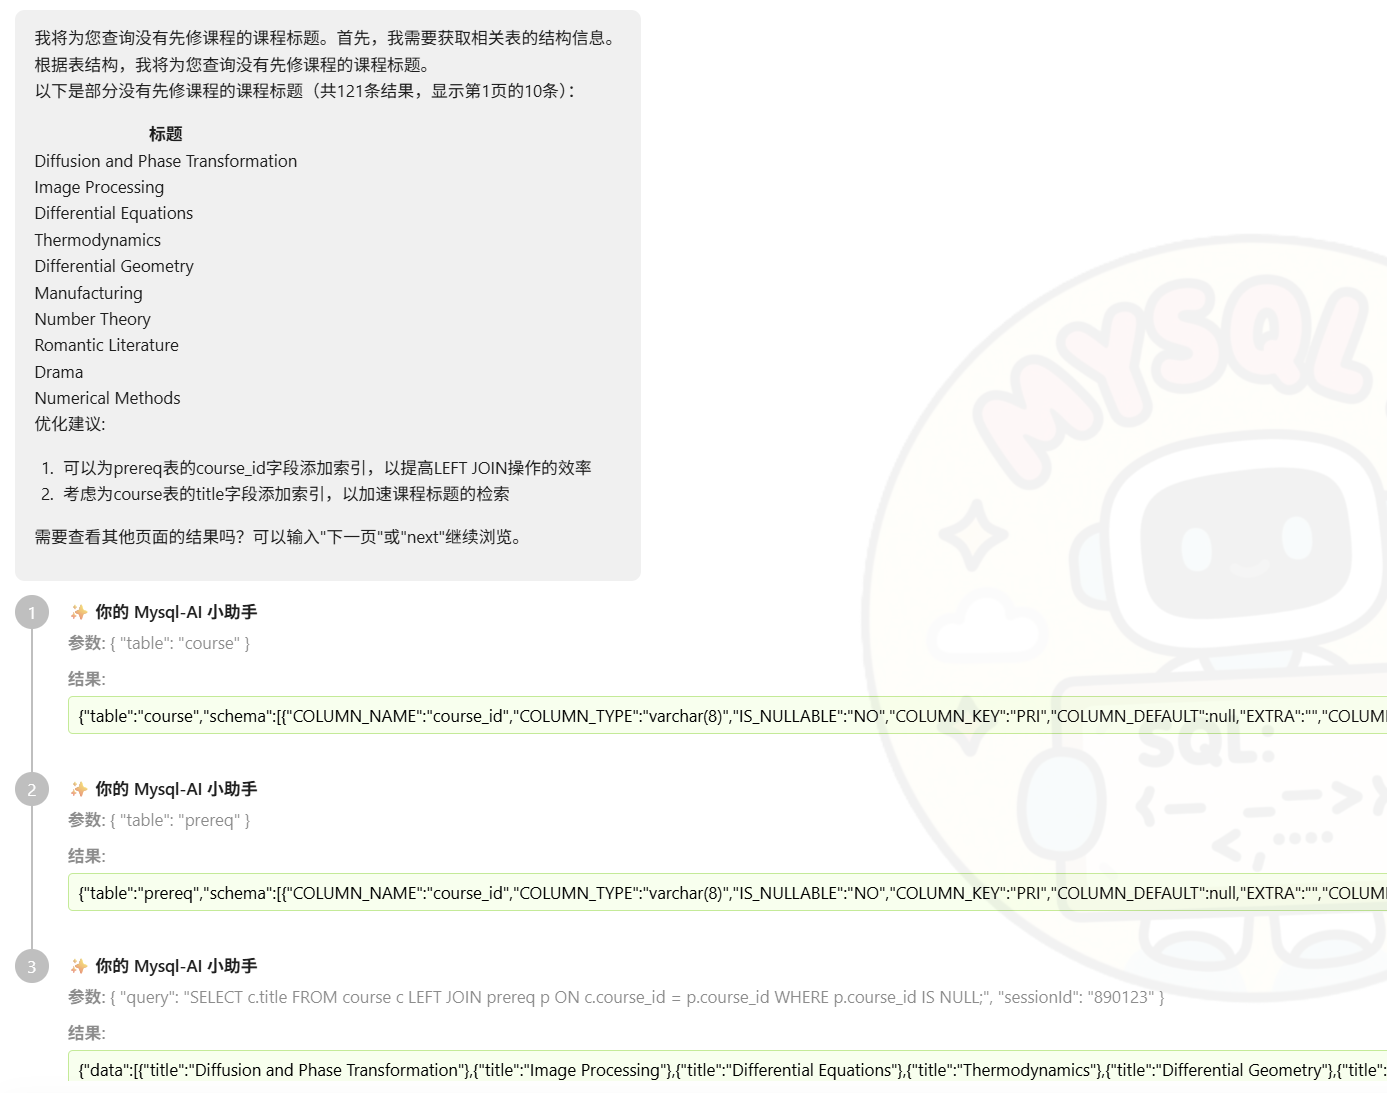
\includegraphics[width=10cm]{./images/13.测试4.jpg}
			\caption{测试4}
		\end{figure}
		
		\item 哪些学生的学分高于他们的平均学分?
		
		\begin{figure}[H]
			\centering
			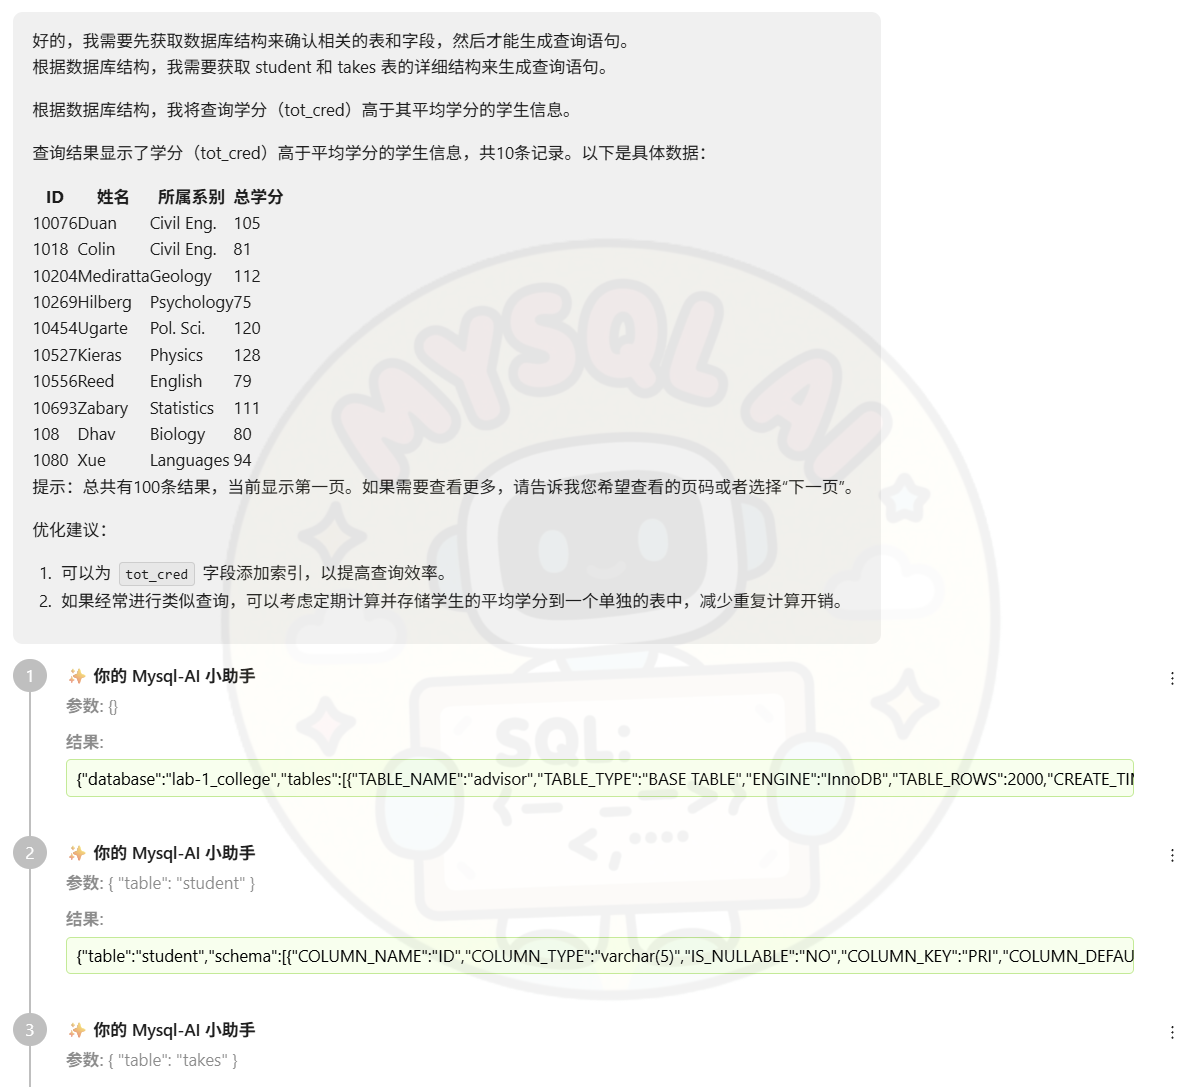
\includegraphics[width=10cm]{./images/14.测试5.jpg}
			\caption{测试5}
		\end{figure}
	\end{enumerate}\textbf{}
	
	\section{遇到的困难与解决方法}
	
	\subsection{MCP服务部署与连接问题}
	\begin{itemize}
		\item \textbf{困难}:
		\begin{itemize}
			\item 初次部署MCP服务时遇到依赖冲突或端口占用问题
			\item 连接MySQL实例时出现认证失败或连接超时
		\end{itemize}
		
		\item \textbf{解决方法}:
		\begin{itemize}
			\item 仔细检查并安装所有必要的依赖项
			\item 使用\texttt{netstat}命令检查端口占用情况,必要时更换端口
			\item 验证MySQL连接字符串的正确性,确保用户名和密码正确
			\item 检查MySQL服务是否正常运行,必要时重启服务
		\end{itemize}
	\end{itemize}
	
	\subsection{大模型API调用问题}
	\begin{itemize}
		\item \textbf{困难}:
		\begin{itemize}
			\item 通义千问API调用配额不足或响应速度慢
			\item API返回的SQL不符合预期格式
			\item 网络连接不稳定导致API调用失败
		\end{itemize}
		
		\item \textbf{解决方法}:
		\begin{itemize}
			\item 申请增加API配额或切换到其他可用的大模型API
			\item 优化prompt设计,增加更明确的指令和示例
			\item 实现API调用重试机制和错误处理
			\item 添加本地缓存机制减少重复API调用
		\end{itemize}
	\end{itemize}
	
	\subsection{SQL生成准确性不足}
	\begin{itemize}
		\item \textbf{困难}:
		\begin{itemize}
			\item 大模型生成的SQL语句存在语法错误
			\item 生成的SQL与数据库schema不匹配
			\item 复杂查询(如多表连接、子查询)生成效果差
		\end{itemize}
		
		\item \textbf{解决方法}:
		\begin{itemize}
			\item 在prompt中明确提供数据库schema信息
			\item 实现SQL语法验证和修正机制
			\item 针对复杂查询设计few-shot prompt,提供示例
			\item 添加SQL执行前的预检查功能
		\end{itemize}
	\end{itemize}
	
	\subsection{查询结果处理问题}
	\begin{itemize}
		\item \textbf{困难}:
		\begin{itemize}
			\item 大量查询结果导致系统性能下降
			\item 结果JSON格式不符合预期
			\item 特殊字符处理不当导致解析错误
		\end{itemize}
		
		\item \textbf{解决方法}:
		\begin{itemize}
			\item 实现分页机制,分批返回查询结果
			\item 严格定义并验证结果JSON的格式规范
			\item 添加结果数据的清洗和转义处理
		\end{itemize}
	\end{itemize}
	
	\subsection{安全控制实现困难}
	\begin{itemize}
		\item \textbf{困难}:
		\begin{itemize}
			\item SQL注入检测机制存在误判或漏判
			\item 敏感字段过滤不全面
			\item 只读控制影响正常查询
		\end{itemize}
		
		\item \textbf{解决方法}:
		\begin{itemize}
			\item 结合正则表达式和关键词列表进行多重检测
			\item 建立完善的敏感字段字典并定期更新
			\item 设计白名单机制,确保只读控制不影响合法查询
		\end{itemize}
	\end{itemize}
	
	\section{其他}
	
	源代码链接:\url{https://github.com/SoftGhostGU/CodeExplorer/tree/main/mysql_%E5%9F%BA%E4%BA%8Emcp}
	
\end{document}
